% Arquivo LaTeX de exemplo de dissertação/tese a ser apresentada à CPG do IME-USP
%
% Criação: Jesús P. Mena-Chalco
% Revisão: Fabio Kon e Paulo Feofiloff
% Adaptação para UTF8, biblatex e outras melhorias: Nelson Lago
%
% Except where otherwise indicated, these files are distributed under
% the MIT Licence. The example text, which includes the tutorial and
% examples as well as the explanatory comments in the source, are
% available under the Creative Commons Attribution International
% Licence, v4.0 (CC-BY 4.0) - https://creativecommons.org/licenses/by/4.0/


%%%%%%%%%%%%%%%%%%%%%%%%%%%%%%%%%%%%%%%%%%%%%%%%%%%%%%%%%%%%%%%%%%%%%%%%%%%%%%%%
%%%%%%%%%%%%%%%%%%%%%%%%%%%%%%% PREÂMBULO LaTeX %%%%%%%%%%%%%%%%%%%%%%%%%%%%%%%%
%%%%%%%%%%%%%%%%%%%%%%%%%%%%%%%%%%%%%%%%%%%%%%%%%%%%%%%%%%%%%%%%%%%%%%%%%%%%%%%%

% A opção twoside (frente-e-verso) significa que a aparência das páginas pares
% e ímpares pode ser diferente. Por exemplo, as margens podem ser diferentes ou
% os números de página podem aparecer à direita ou à esquerda alternadamente.
% Mas nada impede que você crie um documento "só frente" e, ao imprimir, faça
% a impressão frente-e-verso.
%
% Aqui também definimos a língua padrão do documento (a última da lista) e
% línguas adicionais. Para teses do IME, no mínimo português e inglês são
% obrigatórios, porque independentemente da língua principal do texto é
% preciso fornecer o resumo nessas duas línguas. LaTeX aceita alguns nomes
% diferentes para a língua portuguesa; dentre as opções, prefira sempre
% "brazilian" para português brasileiro e "portuguese" para português europeu.
%\documentclass[a4paper,12pt,twoside,brazilian,english]{book}
\documentclass[a4paper,12pt,twoside,english,brazilian]{book}

% O preâmbulo de um documento LaTeX pode ser razoavelmente longo. Neste
% modelo, optamos por reduzi-lo, colocando praticamente tudo do preâmbulo
% nas packages "imegoodies" e "imelooks".
%
% imegoodies carrega diversas packages muito úteis e populares (algumas
% são praticamente obrigatórias, como amsmath, babel, array etc.). É
% uma boa ideia usá-la com outros documentos também. Ela inclui vários
% comentários explicativos e dicas de uso; não tenha medo de alterá-la
% conforme a necessidade.
%
% imelooks carrega algumas packages e configurações que definem a
% aparência do documento; você também pode querer usá-la (ou partes
% dela) com outros documentos para obter as mesmas fontes, margens
% etc. Tal como "imegoodies", pode valer a pena ler os comentários
% e fazer modificações nessa package. Com a opção "thesis", imelooks
% também define os comandos para capa, folha de rosto etc.
\usepackage{imegoodies}
\usepackage[thesis]{imelooks}

%\nocolorlinks % para impressão em P&B

% Diretórios onde estão as figuras; com isso, não é necessário (mas
% é permitido) colocar o caminho completo em \includegraphics. Note
% que a extensão nunca é necessária (mas é permitida), ou seja, o
% resultado é o mesmo com "\includegraphics{figuras/foto.jpeg}",
% "\includegraphics{foto.jpeg}", "\includegraphics{figuras/foto}"
% ou "\includegraphics{foto}".
\graphicspath{{figuras/},{fig/},{logos/},{img/},{images/},{imagens/}}

% Comandos rápidos para mudar de língua:
% \en -> muda para o inglês
% \br -> muda para o português
% \texten{blah} -> o texto "blah" é em inglês
% \textbr{blah} -> o texto "blah" é em português
\babeltags{br = brazilian, en = english}


%%%%%%%%%%%%%%%%%%%%%%%%%%%%%%%%%%%%%%%%%%%%%%%%%%%%%%%%%%%%%%%%%%%%%%%%%%%%%%%%
%%%%%%%%%%%%%%%%%%%%%%%%%%%%%%%%%% METADADOS %%%%%%%%%%%%%%%%%%%%%%%%%%%%%%%%%%%
%%%%%%%%%%%%%%%%%%%%%%%%%%%%%%%%%%%%%%%%%%%%%%%%%%%%%%%%%%%%%%%%%%%%%%%%%%%%%%%%

% O arquivo com os dados bibliográficos para biblatex; você pode usar
% este comando mais de uma vez para acrescentar múltiplos arquivos
\addbibresource{bibliografia.bib}

% Este comando permite acrescentar itens à lista de referências sem incluir
% uma referência de fato no texto (pode ser usado em qualquer lugar do texto)
%\nocite{bronevetsky02,schmidt03:MSc, FSF:GNU-GPL, CORBA:spec, MenaChalco08}
% Com este comando, todos os itens do arquivo .bib são incluídos na lista
% de referências
%\nocite{*}

% É possível definir como determinadas palavras podem (ou não) ser
% hifenizadas; no entanto, a hifenização automática geralmente funciona bem
\babelhyphenation{documentclass latexmk soft-ware clsguide} % todas as línguas
\babelhyphenation[brazilian]{Fu-la-no}
\babelhyphenation[english]{what-ever}

% Estes comandos definem o título e autoria do trabalho e devem sempre ser
% definidos, pois além de serem utilizados para criar a capa, também são
% armazenados nos metadados do PDF. O subtítulo é opcional.
\title{USP Kart}[jogo de corrida em OpenGL estilo Mario Kart]
\translatedtitle{USP Kart}[OpenGL racing game in the style of Mario Kart]

\author{Pedro Zamecki Andrade}

\def\profa{Prof\kern.02em.\kern-.07emª\kern.07em}
\def\dra{Dr\kern-.04em.\kern-.11emª\kern.07em}

% Para TCCs, este comando define o supervisor
\orientador{Prof. Dr. Paulo Andre Vechiatto de Miranda}

\banca{
  Prof. Dr. Paulo Andre Vechiato de Miranda (orientador) -- IME-USP [sem ponto final],
}

% A página de rosto da versão para depósito (ou seja, a versão final
% antes da defesa) deve ser diferente da página de rosto da versão
% definitiva (ou seja, a versão final após a incorporação das sugestões
% da banca).
\tipotese{
  %mestrado,
  %doutorado,
  tcc,
  %definitiva, % É a versão para defesa ou a versão definitiva?
  %quali, % É qualificação?
  programa={Ciência da Computação},
}

\defesa{
  local={São Paulo},
  data=2024-11-08, % YYYY-MM-DD
}

% A licença do seu trabalho. Use CC-BY, CC-BY-NC, CC-BY-ND, CC-BY-SA,
% CC-BY-NC-SA ou CC-BY-NC-ND para escolher a licença Creative Commons
% correspondente (o sistema insere automaticamente o texto da licença).
% Se quiser estabelecer regras diferentes para o uso de seu trabalho,
% converse com seu orientador e coloque o texto da licença aqui, mas
% observe que apenas TCCs sob alguma licença Creative Commons serão
% acrescentados ao BDTA. Se você tem alguma intenção de publicar o
% trabalho comercialmente no futuro, sugerimos a licença CC-BY-NC-ND.
%
%\direitos{CC-BY-NC-ND}
%
\direitos{Autorizo a reprodução e divulgação total ou parcial deste
          trabalho, por qualquer meio convencional ou eletrônico,
          para fins de estudo e pesquisa, desde que citada a fonte.}

\direitos{I authorize the complete or partial reproduction and disclosure
          of this work by any conventional or electronic means for study
          and research purposes, provided that the source is acknowledged.}

\direitos{CC-BY}

% Para gerar a ficha catalográfica, acesse https://fc.ime.usp.br/,
% preencha o formulário e escolha a opção "Gerar Código LaTeX".
% Basta copiar e colar o resultado aqui.
\fichacatalografica{}


%%%%%%%%%%%%%%%%%%%%%%%%%%%%%%%%%%%%%%%%%%%%%%%%%%%%%%%%%%%%%%%%%%%%%%%%%%%%%%%%
%%%%%%%%%%%%%%%%%%%%%%% AQUI COMEÇA O CONTEÚDO DE FATO %%%%%%%%%%%%%%%%%%%%%%%%%
%%%%%%%%%%%%%%%%%%%%%%%%%%%%%%%%%%%%%%%%%%%%%%%%%%%%%%%%%%%%%%%%%%%%%%%%%%%%%%%%

\begin{document}

%%%%%%%%%%%%%%%%%%%%%%%%%%% CAPA E PÁGINAS INICIAIS %%%%%%%%%%%%%%%%%%%%%%%%%%%%

% Aqui começa o conteúdo inicial que aparece antes do capítulo 1, ou seja,
% página de rosto, resumo, sumário etc. O comando frontmatter faz números
% de página aparecem em algarismos romanos ao invés de arábicos e
% desabilita a contagem de capítulos.
\frontmatter

\pagestyle{plain}

\onehalfspacing{}

\maketitle % capa e folha de rosto

%%%%%%%%%%%%%%%% DEDICATÓRIA, AGRADECIMENTOS, RESUMO/ABSTRACT %%%%%%%%%%%%%%%%%%

\begin{dedicatoria}
Eu dedico este trabalho à minha família, amigos e professores que me guiaram e apoiaram durante a graduação. Em especial à minha namorada que esteve do meu lado nesses momentos difíceis e me ajudou a superar cada obstáculo.

\end{dedicatoria}

% Reinicia o contador de páginas (a próxima página recebe o número "i") para
% que a página da dedicatória não seja contada.
\pagenumbering{roman}

% Agradecimentos:
% Se o candidato não quer fazer agradecimentos, deve simplesmente eliminar
% esta página. A epígrafe, obviamente, é opcional; é possível colocar
% epígrafes em todos os capítulos. O comando "\chapter*" faz esta seção
% não ser incluída no sumário.
\chapter*{Agradecimentos}
\epigrafe{Bad programmers worry about the code. Good programmers worry about data structures and their relationships.}{Linus Torvalds}

Eu gostaria de agradecer a todos que estiveram comigo na minha graduação,
todos aqueles que me ajudaram a superar cada limite e dificuldade durante esses anos.

%!TeX root=../tese.tex
%("dica" para o editor de texto: este arquivo é parte de um documento maior)
% para saber mais: https://tex.stackexchange.com/q/78101

% As palavras-chave são obrigatórias, em português e em inglês, e devem ser
% definidas antes do resumo/abstract. Acrescente quantas forem necessárias.
\palavraschave{Jogo, Corrida, OpenGL, Kart}

\keywords{Game, Racing, OpenGL, Kart}

% O resumo é obrigatório, em português e inglês. Estes comandos também
% geram automaticamente a referência para o próprio documento, conforme
% as normas sugeridas da USP.
\resumo{
Este trabalho apresenta o desenvolvimento de USP Kart, um jogo eletrônico inspirado no clássico Mario Kart. O projeto combina elementos de entretenimento e desafios técnicos, integrando conceitos avançados de computação gráfica e algoritmos de busca de caminhos.

Utilizando bibliotecas amplamente empregadas no desenvolvimento de gráficos 3D, como OpenGL, GLEW, GLFW, ASSIMP e GLM, USP Kart foi implementado em C++ para explorar os recursos de paralelismo da linguagem. Este recurso foi essencial para gerenciar múltiplos corredores controlados por computador, representando o algoritmo programado para competir no jogo. O comportamento desses agentes foi desenvolvido utilizando o algoritmo A*, que permite o cálculo eficiente do caminho mais curto até a próxima linha de controle, mesmo em cenários dinâmicos e complexos.

A estética do jogo foi criada do zero, com uma direção artística que homenageia a Universidade de São Paulo (USP) e o Instituto de Matemática e Estatística (IME), incluindo a representação da mascote Fluffy. Essa identidade visual foi projetada para proporcionar uma experiência imersiva e personalizada para os jogadores, utilizando modelos de representação de carros com o \textit{bicycle model}\index{Língua estrangeira}, modelo de representação de carros.

O projeto também aborda os desafios encontrados na integração entre gráficos, física, ferramentas para desenvolvimento e cálculos de descoberta de caminhos em tempo real, além de destacar os benefícios do uso de técnicas de programação modernas e bibliotecas de código aberto. Por fim, USP Kart busca não apenas oferecer um produto jogável, mas também servir como estudo de caso para a aplicação prática de conceitos de computação gráfica, paralelismo e algoritmos de busca.
}
\abstract{
This work presents the development of USP Kart, an electronic game inspired by the classic Mario Kart. The project combines elements of entertainment and technical challenges, integrating advanced concepts of computer graphics and pathfinding algorithms.

Using libraries widely employed in the development of 3D graphics, such as OpenGL, GLEW, GLFW, ASSIMP and GLM, USP Kart was implemented in C++ to explore the language's parallelism features. This feature was essential to manage multiple computer-controlled racers, representing the programmed algorithm to compete in the game. The behavior of these agents was developed using the A* algorithm, which allows the efficient calculation of the shortest path to the next checkpoint, even in dynamic and complex scenarios.

The game's aesthetics were created from scratch, with an artistic direction that pays homage to the University of São Paulo (USP) and the Institute of Mathematics and Statistics (IME), including the representation of the mascot Fluffy. This visual identity was designed to provide an immersive and personalized experience for players, using car representation models with the 'bicycle model', a car representation model.

The project also addresses the challenges encountered in the integration between graphics, physics, development tools, and real-time pathfinding calculations, as well as highlighting the benefits of using modern programming techniques and open-source libraries. Finally, USP Kart seeks not only to offer a playable product but also to serve as a case study for the practical application of computer graphics, parallelism, and search algorithms concepts.
}



%%%%%%%%%%%%%%%%%%%%%%%%%%% LISTAS DE FIGURAS ETC. %%%%%%%%%%%%%%%%%%%%%%%%%%%%%

% Como as listas que se seguem podem não incluir uma quebra de página
% obrigatória, inserimos uma quebra manualmente aqui.
\cleardoublepage

% Todas as listas são opcionais; Usando "\chapter*" elas não são incluídas
% no sumário. As listas geradas automaticamente também não são incluídas por
% conta das opções "notlot" e "notlof" que usamos para a package tocbibind.

% Normalmente, "\chapter*" faz o novo capítulo iniciar em uma nova página, e as
% listas geradas automaticamente também por padrão ficam em páginas separadas.
% Como cada uma destas listas é muito curta, não faz muito sentido fazer isso
% aqui, então usamos este comando para desabilitar essas quebras de página.
% Se você preferir, comente as linhas com esse comando e des-comente as linhas
% sem ele para criar as listas em páginas separadas. Observe que você também
% pode inserir quebras de página manualmente (com \clearpage, veja o exemplo
% mais abaixo).
\newcommand\disablenewpage[1]{{\let\clearpage\par\let\cleardoublepage\par #1}}

% Nestas listas, é melhor usar "raggedbottom" (veja basics.tex). Colocamos
% a opção correspondente e as listas dentro de um grupo para ativar
% raggedbottom apenas temporariamente.
\bgroup
\raggedbottom

%%%%% Listas criadas manualmente

%\chapter*{Lista de abreviaturas}
\disablenewpage{\chapter*{Lista de abreviaturas}}

\begin{tabular}{rl}
   IME & Instituto de Matemática e Estatística\\
   USP & Universidade de São Paulo \\
   SAT & Separating Axis Theorem \\
\end{tabular}

%\chapter*{Lista de símbolos}
\disablenewpage{\chapter*{Lista de símbolos}}

\begin{tabular}{rl}
\end{tabular}

% Quebra de página manual
\clearpage

%%%%% Listas criadas automaticamente

% Você pode escolher se quer ou não permitir a quebra de página
%\listoffigures
\disablenewpage{\listoffigures}

% Você pode escolher se quer ou não permitir a quebra de página
%\listoftables
\disablenewpage{\listoftables}

% Esta lista é criada "automaticamente" pela package float quando
% definimos o novo tipo de float "program" (em utils.tex)
% Você pode escolher se quer ou não permitir a quebra de página
%\listof{program}{\programlistname}
\disablenewpage{\listof{program}{\programlistname}}

% Sumário (obrigatório)
\tableofcontents

\egroup % Final de "raggedbottom"

% Referências indiretas ("x", veja "y") para o índice remissivo (opcionais,
% pois o índice é opcional). É comum colocar esses itens no final do documento,
% junto com o comando \printindex, mas em alguns casos isso torna necessário
% executar texindy (ou makeindex) mais de uma vez, então colocar aqui é melhor.
\index{Inglês|see{Língua estrangeira}}
\index{Figuras|see{Floats}}
\index{Tabelas|see{Floats}}
\index{Código-fonte|see{Floats}}
\index{Subcaptions|see{Subfiguras}}
\index{Sublegendas|see{Subfiguras}}
\index{Equações|see{Modo matemático}}
\index{Fórmulas|see{Modo matemático}}
\index{Rodapé, notas|see{Notas de rodapé}}
\index{Captions|see{Legendas}}
\index{Versão original|see{Tese/Dissertação, versões}}
\index{Versão corrigida|see{Tese/Dissertação, versões}}
\index{Palavras estrangeiras|see{Língua estrangeira}}
\index{Floats!Algoritmo|see{Floats, ordem}}


%%%%%%%%%%%%%%%%%%%%%%%%%%%%%%%% CAPÍTULOS %%%%%%%%%%%%%%%%%%%%%%%%%%%%%%%%%%%%%

% Aqui vai o conteúdo principal do trabalho, ou seja, os capítulos que compõem
% a dissertação/tese. O comando mainmatter reinicia a contagem de páginas,
% modifica a numeração para números arábicos e ativa a contagem de capítulos.
\mainmatter

\pagestyle{mainmatter}

% Espaçamento simples
\singlespacing

% A introdução não tem número de capítulo, então os cabeçalhos também não
\pagestyle{unnumberedchapter}
%!TeX root=../tese.tex
%("dica" para o editor de texto: este arquivo é parte de um documento maior)
% para saber mais: https://tex.stackexchange.com/q/78101

%% ------------------------------------------------------------------------- %%

% "\chapter" cria um capítulo com número e o coloca no sumário; "\chapter*"
% cria um capítulo sem número e não o coloca no sumário. A introdução não
% deve ser numerada, mas deve aparecer no sumário. Por conta disso, este
% modelo define o comando "\chapter**".
\chapter**{Introdução}
\label{cap:introducao}

\enlargethispage{.5\baselineskip}

A indústria de jogos eletrônicos é um dos setores que mais cresce globalmente, movimentando bilhões de dólares e impactando diversas áreas, desde a tecnologia até a cultura popular. Com mais de quarenta anos de história, os jogos eletrônicos evoluíram de experiências simples em 2D para produções altamente complexas e imersivas em 3D, alavancadas por avanços tecnológicos e pela criatividade de desenvolvedores ao redor do mundo. Gêneros como aventura, RPG (\textit{Role-playing game}, ou em português 'jogo de interpretação de papéis'), FPS (\textit{First Person Shooter}, ou em português 'Tiro em primeira pessoa') e corrida se consolidaram como pilares dessa indústria, atraindo uma ampla gama de jogadores.

No gênero de jogos de corrida, títulos como \textit{Mario Kart}\index{Língua estrangeira} se destacam não apenas pela jogabilidade divertida e acessível, mas também pela capacidade de reunir amigos e familiares em competições intensas e, por vezes, imprevisíveis. Lançado originalmente em 1992, \textit{Mario Kart} (\cite{marioKart}) redefiniu o gênero ao introduzir elementos de combate e interação dinâmica, como o uso de itens para atrapalhar os adversários. Esse modelo de jogo se mostrou extremamente popular e influente, servindo de inspiração para outros títulos como \textit{Crash Team Racing}\index{Língua estrangeira} (\cite{crashTeamRacing}), \textit{Sonic \& All-Stars Racing}\index{Língua estrangeira} (\cite{sonicAllStars}) e \textit{Blur}\index{Língua estrangeira} (\cite{blur}). Ademais, estudos recentes mostram que \textit{Mario Kart}\index{Língua estrangeira} é considerado um dos jogos mais estressantes pelos jogadores (\cite{stressful:bonusFinder}), devido às viradas de sorte e à competitividade elevada, aspectos que o tornam cativante e memorável.

\section**{Motivação}
Apesar do sucesso internacional desse estilo de jogo, o mercado brasileiro ainda carece de produções relevantes no segmento. A indústria nacional de jogos tem mostrado crescimento expressivo, mas a maior parte dos títulos lançados se concentra em gêneros como aventura, \textit{indie}\index{Língua estrangeira} e simuladores. Jogos de corrida com o apelo dinâmico de \textit{Mario Kart}\index{Língua estrangeira}, especialmente aqueles com elementos culturais que reflitam a identidade brasileira, são raros ou inexistentes. Esse cenário evidencia uma lacuna que pode ser explorada por desenvolvedores locais, tanto para diversificar o mercado quanto para criar experiências que dialoguem com o público brasileiro.

O presente trabalho apresenta uma primeira contribuição para suprir a carência de títulos nacionais sobre o tema com o desenvolvimento do  \textit{USP Kart}, um jogo de corrida inspirado em \textit{Mario Kart}\index{Língua estrangeira}, mas com uma identidade fortemente vinculada à Universidade de São Paulo (USP) e ao Instituto de Matemática e Estatística (IME). Além de oferecer uma experiência de jogo envolvente, o projeto também explora soluções tecnológicas inovadoras e visa destacar o potencial criativo da indústria brasileira de jogos. A partir dessa monografia, espera-se não apenas preencher a lacuna existente no mercado nacional, mas também contribuir para o avanço do conhecimento técnico e artístico no desenvolvimento de jogos eletrônicos no Brasil.

\section**{Objetivos}
\label{sec:consideracoes_preliminares}
O objetivo principal deste trabalho é desenvolver o \textit{USP Kart}, um jogo eletrônico de corrida inspirado no clássico \textit{Mario Kart}, com características únicas que valorizem a identidade cultural e acadêmica da Universidade de São Paulo (USP). Para alcançar essa meta, os seguintes objetivos específicos são estabelecidos\:
\begin{itemize}
\item Criar uma experiência de jogo imersiva e divertida, utilizando mecânicas de corrida e combate dinâmicas que remetam a jogos consagrados do gênero, como \textit{Mario Kart}.

\item Desenvolver a estética do jogo com temática inspirada na USP, com ênfase especial no Instituto de Matemática e Estatística (IME), incluindo referências visuais e conceituais à mascote Fluffy e outros elementos distintivos.

\item Implementar tecnologias modernas de computação gráfica e inteligência artificial para garantir a qualidade técnica e inovadora do jogo.

\item Explorar o potencial de jogos eletrônicos para destacar a cultura universitária brasileira e preencher lacunas no mercado nacional de jogos eletrônicos.
\end{itemize}

\enlargethispage{.5\baselineskip}

\section**{Metodologia}

O desenvolvimento do \textit{USP Kart} foi desenvolvido por uma abordagem estruturada que combina aspectos técnicos e criativos. O trabalho foi conduzido em etapas distintas, conforme descrito a seguir\:

\begin{itemize}

\item \textbf{Criação de um motor gráfico do zero em C++:} o jogo foi desenvolvido utilizando um motor gráfico proprietário, desenvolvido especificamente para atender às necessidades do projeto. Essa abordagem permitiu maior controle sobre os detalhes técnicos, possibilitando assim a exploração de funcionalidades customizadas.
    
\item \textbf{Utilização do OpenGL:} o OpenGL foi empregado como base para a renderização gráfica, garantindo alto desempenho e flexibilidade no desenvolvimento dos recursos visuais do jogo. A escolha dessa tecnologia permite a criação de gráficos 3D imersivos e de alta qualidade.
    
\item \textbf{Suporte multiplataforma:} o jogo foi projetado para ser compatível com múltiplos sistemas operacionais, incluindo Windows, macOS e Linux. Isso foi alcançado por práticas de programação portáveis e pela utilização de bibliotecas compatíveis com diferentes plataformas.
    
\item \textbf{Integração de elementos estéticos e culturais:} durante o desenvolvimento, foi dado um enfoque especial à estilização do jogo com temas relacionados à USP e ao IME, criando uma identidade visual e narrativa que destacam elementos culturais e acadêmicos.
    
\end{itemize}
    
Essa metodologia visa assegurar que o \textit{USP Kart} seja tecnicamente robusto, esteticamente atrativo e acessível a um público diversificado.
\pagestyle{mainmatter}
\chapter{Indústria brasileira de Jogos Eletrônicos}

A indústria de jogos no Brasil tem se consolidado como um dos maiores mercados consumidores do mundo, ocupando atualmente a quinta posição global em consumo de jogos eletrônicos. Dados recentes apontam que 89,8\% da população brasileira consome jogos regularmente (\cite{internetGame:share}), utilizando dispositivos móveis, consoles e computadores como principais plataformas. Essa alta adesão reflete a popularidade dos jogos eletrônicos no país, que ultrapassaram a barreira do entretenimento e se tornaram parte do cotidiano de grande parte dos brasileiros.

Entretanto, apesar da expressiva participação no consumo, o Brasil enfrenta desafios significativos quando se trata de publicação de jogos. Publicadoras de jogos, responsáveis por financiar, distribuir e promover os títulos no mercado, desempenham um papel crucial no sucesso de um jogo. Essas empresas frequentemente definem o alcance e o impacto que um título pode ter globalmente. Contudo, o Brasil não figura nem entre os dez principais países que mais publicam jogos (\cite{publishers:country}), evidenciando uma discrepância significativa entre o consumo e a produção nacional.

\begin{figure}[H]
    \centering
    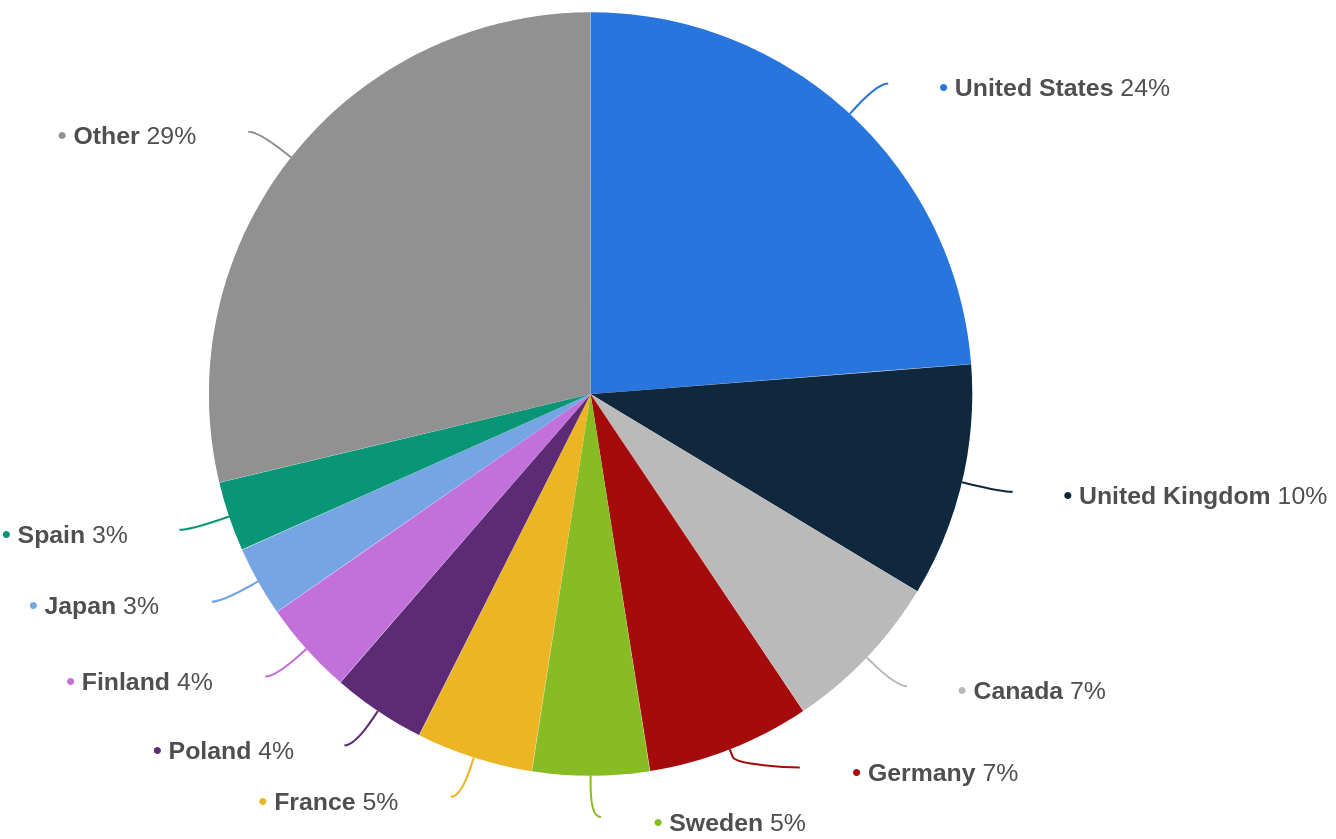
\includegraphics[width=0.8\textwidth]{figuras/Devs by Country.png}
    \caption{Distribuição de publicadoras de jogos por país. Fonte: \cite{publishers:country}}
    \label{fig:jogos-brasil}
\end{figure}

\section{História e evolução}
Historicamente, a indústria brasileira de jogos foca em títulos independentes e projetos de menor escala, devido às limitações de financiamento e infraestrutura. Embora existam exemplos notáveis de jogos brasileiros que alcançaram sucesso internacional, como \textit{Horizon Chase Turbo}\label{Língua estrangeira} e \textit{Chroma Squad}, os gêneros mais explorados tendem a ser aventura, RPG e simuladores, enquanto outros segmentos, como o de jogos de corrida no estilo Mario Kart (com elementos de trapaça e apelo competitivo), ainda são pouco explorados.

Esse cenário oferece tanto desafios quanto, oportunidades para desenvolvedores brasileiros. De um lado, a falta de grandes publicadoras locais dificulta o alcance global dos títulos nacionais. Por outro lado, o imenso potencial criativo e a crescente comunidade de desenvolvedores no Brasil sugerem que o mercado pode se expandir significativamente, caso receba os investimentos e apoios necessários. Além disso, a criação de jogos que dialoguem com a identidade cultural brasileira pode ser um diferencial estratégico, atraindo tanto o público nacional quanto internacional.

Ao propor o desenvolvimento do \textit{USP Kart}, este trabalho busca não apenas explorar as possibilidades técnicas e criativas do desenvolvimento de jogos, mas também contribuir para a diversificação do mercado nacional. O objetivo é oferecer uma experiência de jogo de alta qualidade que valorize elementos culturais e acadêmicos brasileiros, demonstrando que o país possui capacidade técnica e artística para competir em segmentos atualmente pouco explorados.

\section{Títulos nacionais}
Apesar dos desafios enfrentados pela indústria brasileira de jogos, diversos títulos nacionais têm se destacado nos últimos anos, tanto no mercado interno quanto no internacional. Jogos como \textit{Horizon Chase Turbo}, \textit{Chroma Squad}, \textit{Dandara} e \textit{Aritana e a Pena da Harpia} são exemplos de produções brasileiras que conquistaram reconhecimento global, recebendo prêmios e críticas positivas da imprensa especializada.

Esses títulos demonstram a diversidade e a qualidade dos jogos produzidos no Brasil, abordando temas variados e explorando mecânicas inovadoras. Além disso, esses jogos frequentemente refletem a cultura e a identidade brasileira, apresentando elementos visuais e narrativos que dialogam com o público nacional e internacional. Um exemplo notável é o "Horizon Chase Turbo - Senna Forever", que homenageia o piloto brasileiro Ayrton Senna e destaca elementos culturais brasileiros.

\begin{figure}[H]
    \centering
    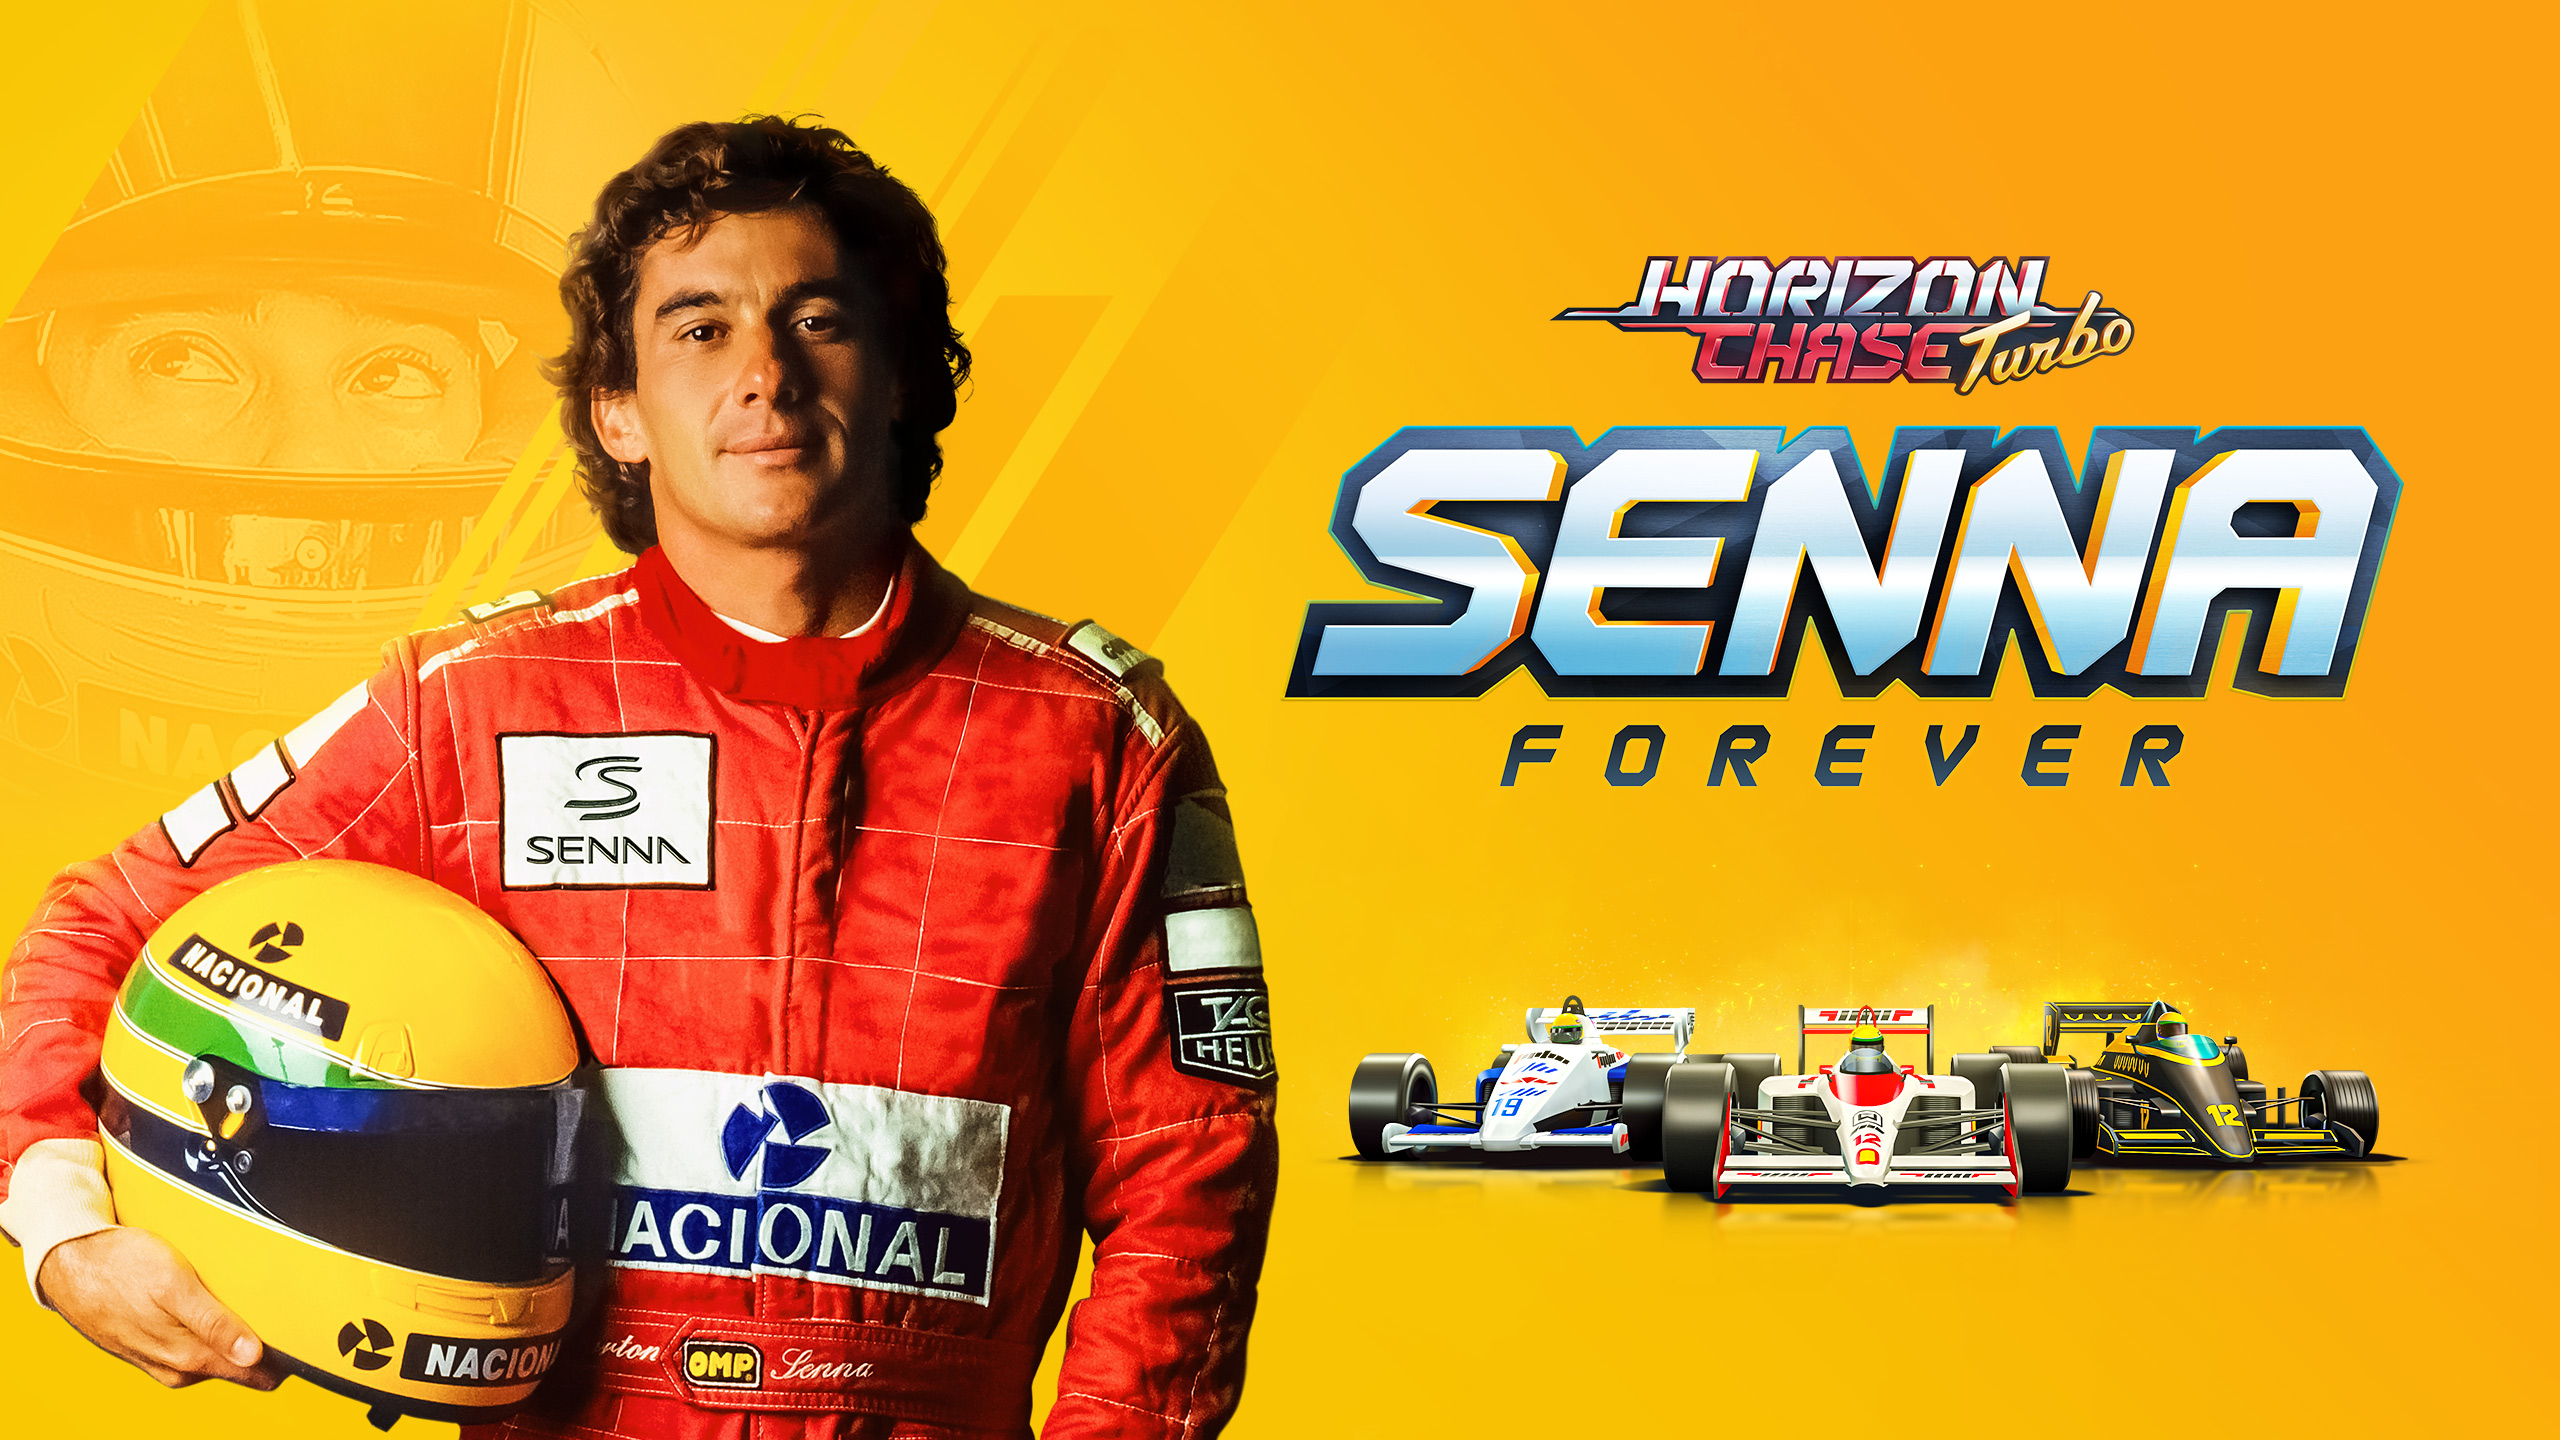
\includegraphics[width=0.8\textwidth]{figuras/Horizon Chase Turbo - Senna.jpg}
    \caption{Homenagem ao piloto brasileiro, Ayrton Senna no jogo Horizon Chase Turbo. \cite{horizonChaseTurbo}}
    \label{fig:horizon-chase-turbo-senna}
\end{figure}

\subsection{Horizon Chase Turbo}
\textit{Horizon Chase Turbo} é um jogo de corrida desenvolvido pela Aquiris Game Studio, lançado em 2018 para múltiplas plataformas. Inspirado em clássicos dos anos 80 e 90, como \textit{Out Run} e \textit{Top Gear}, o jogo combina gráficos 3D modernos com jogabilidade arcade, oferecendo uma experiência nostálgica e desafiadora para os jogadores.

Como o \textit{USP Kart}, \textit{Horizon Chase Turbo} é um jogo de corrida que busca recriar a diversão e a emoção dos jogos clássicos do gênero. A estética retrô e a jogabilidade acessível são elementos-chave do jogo, que conquistou tanto fãs de longa data quanto novos jogadores.

Apesar das semelhanças, \textit{Horizon Chase Turbo} e \textit{USP Kart} diferem em suas abordagens como um jogo de corrida, sendo o gênero de corridas em Kart um subgênero de jogos de corrida que se destaca por sua jogabilidade acessível e dinâmica. Enquanto \textit{Horizon Chase Turbo} foca em corridas de carros clássicos em pistas realistas, \textit{USP Kart} explora mecânicas de combate e interação entre jogadores, inspiradas em títulos como \textit{Mario Kart}.

\begin{figure}[H]
    \centering
    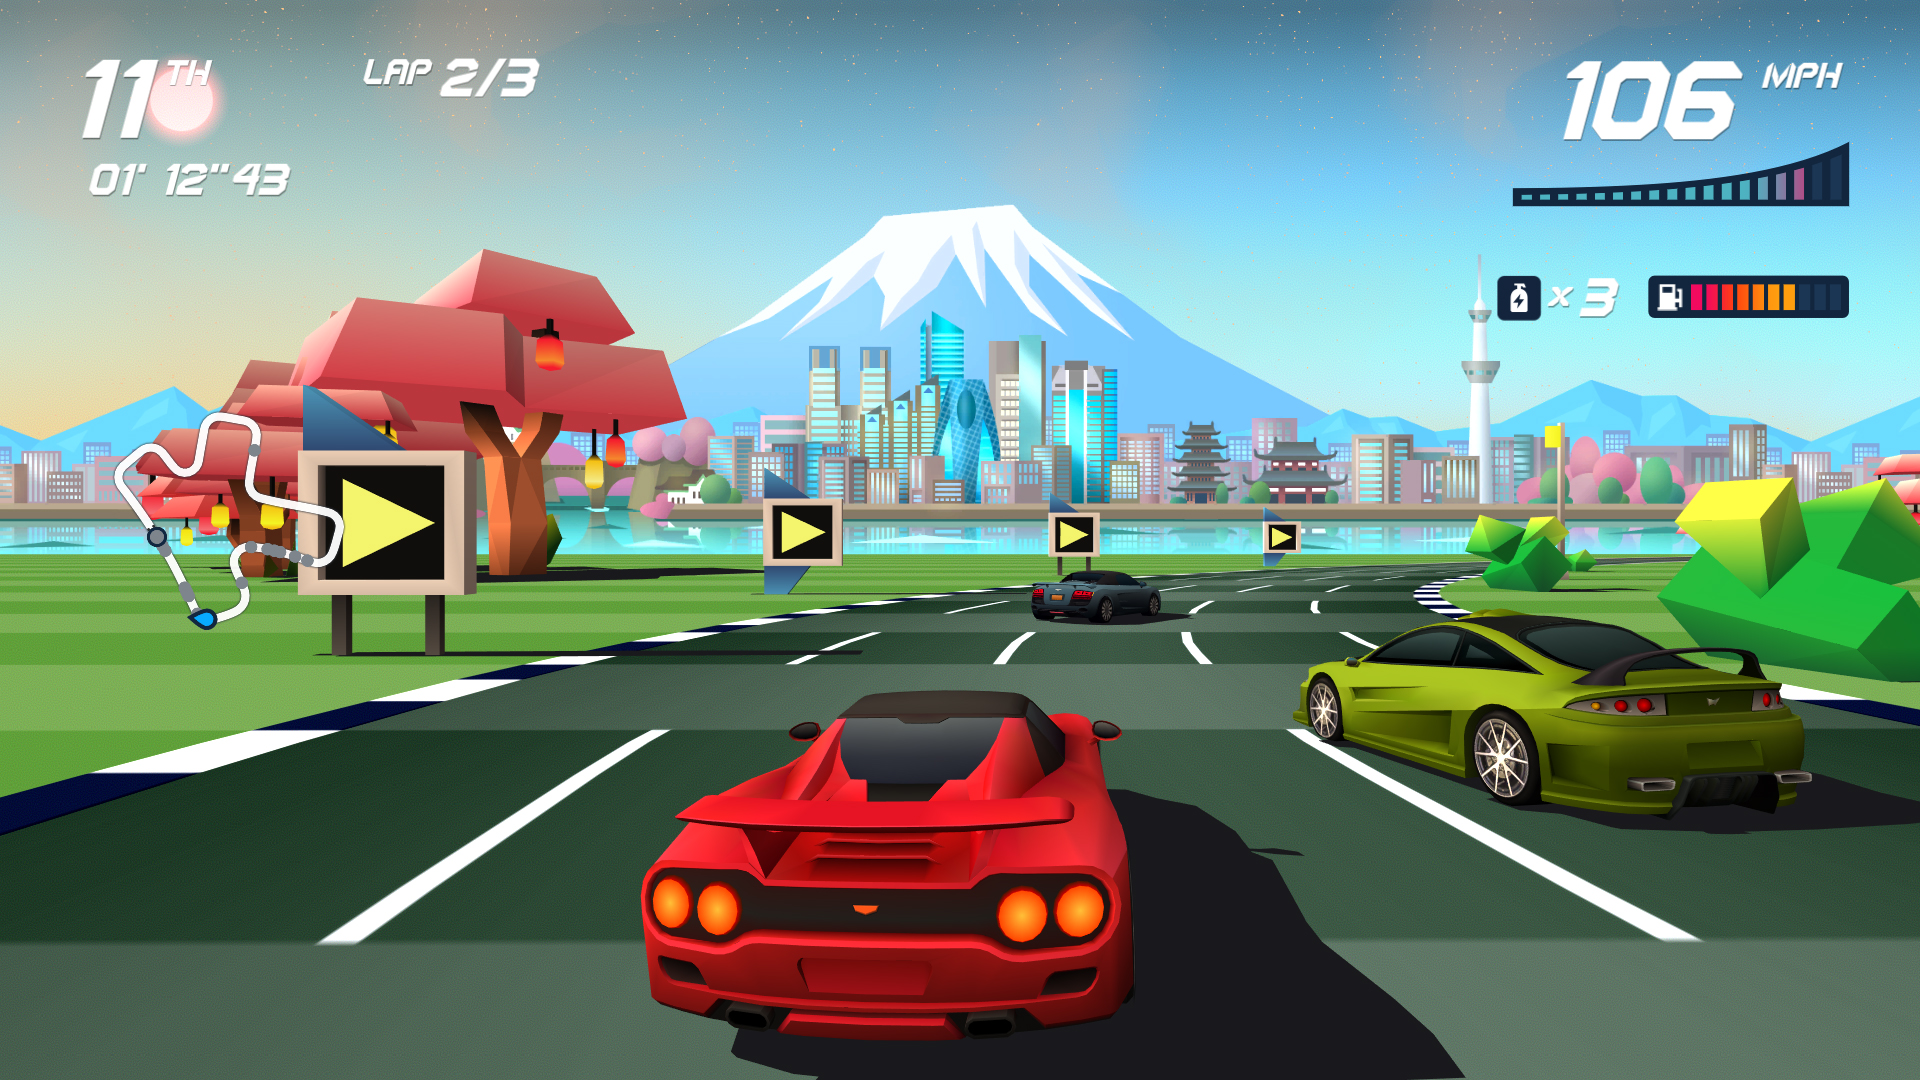
\includegraphics[width=0.8\textwidth]{figuras/Horizon Chase Turbo.jpeg}
    \caption{Horizon Chase Turbo. Fonte: \cite{horizonChaseTurbo}}
    \label{fig:horizon-chase-turbo}
\end{figure}

\subsection{Chroma Squad}
\textit{Chroma Squad} é um jogo de estratégia desenvolvido pela Behold Studios, lançado em 2015 para múltiplas plataformas. O jogo coloca o jogador no papel de um produtor de um programa de TV sobre super-heróis, permitindo que ele controle os personagens, cenários e enredos das batalhas.

\textit{Chroma Squad} é um exemplo de jogo brasileiro que se destaca pela criatividade e originalidade de sua proposta. A mistura de elementos de estratégia, simulação e RPG, combinada com uma narrativa envolvente e humorística, conquistou tanto a crítica quanto o público, tornando-se um dos títulos mais populares da Behold Studios.

\begin{figure}[H]
    \centering
    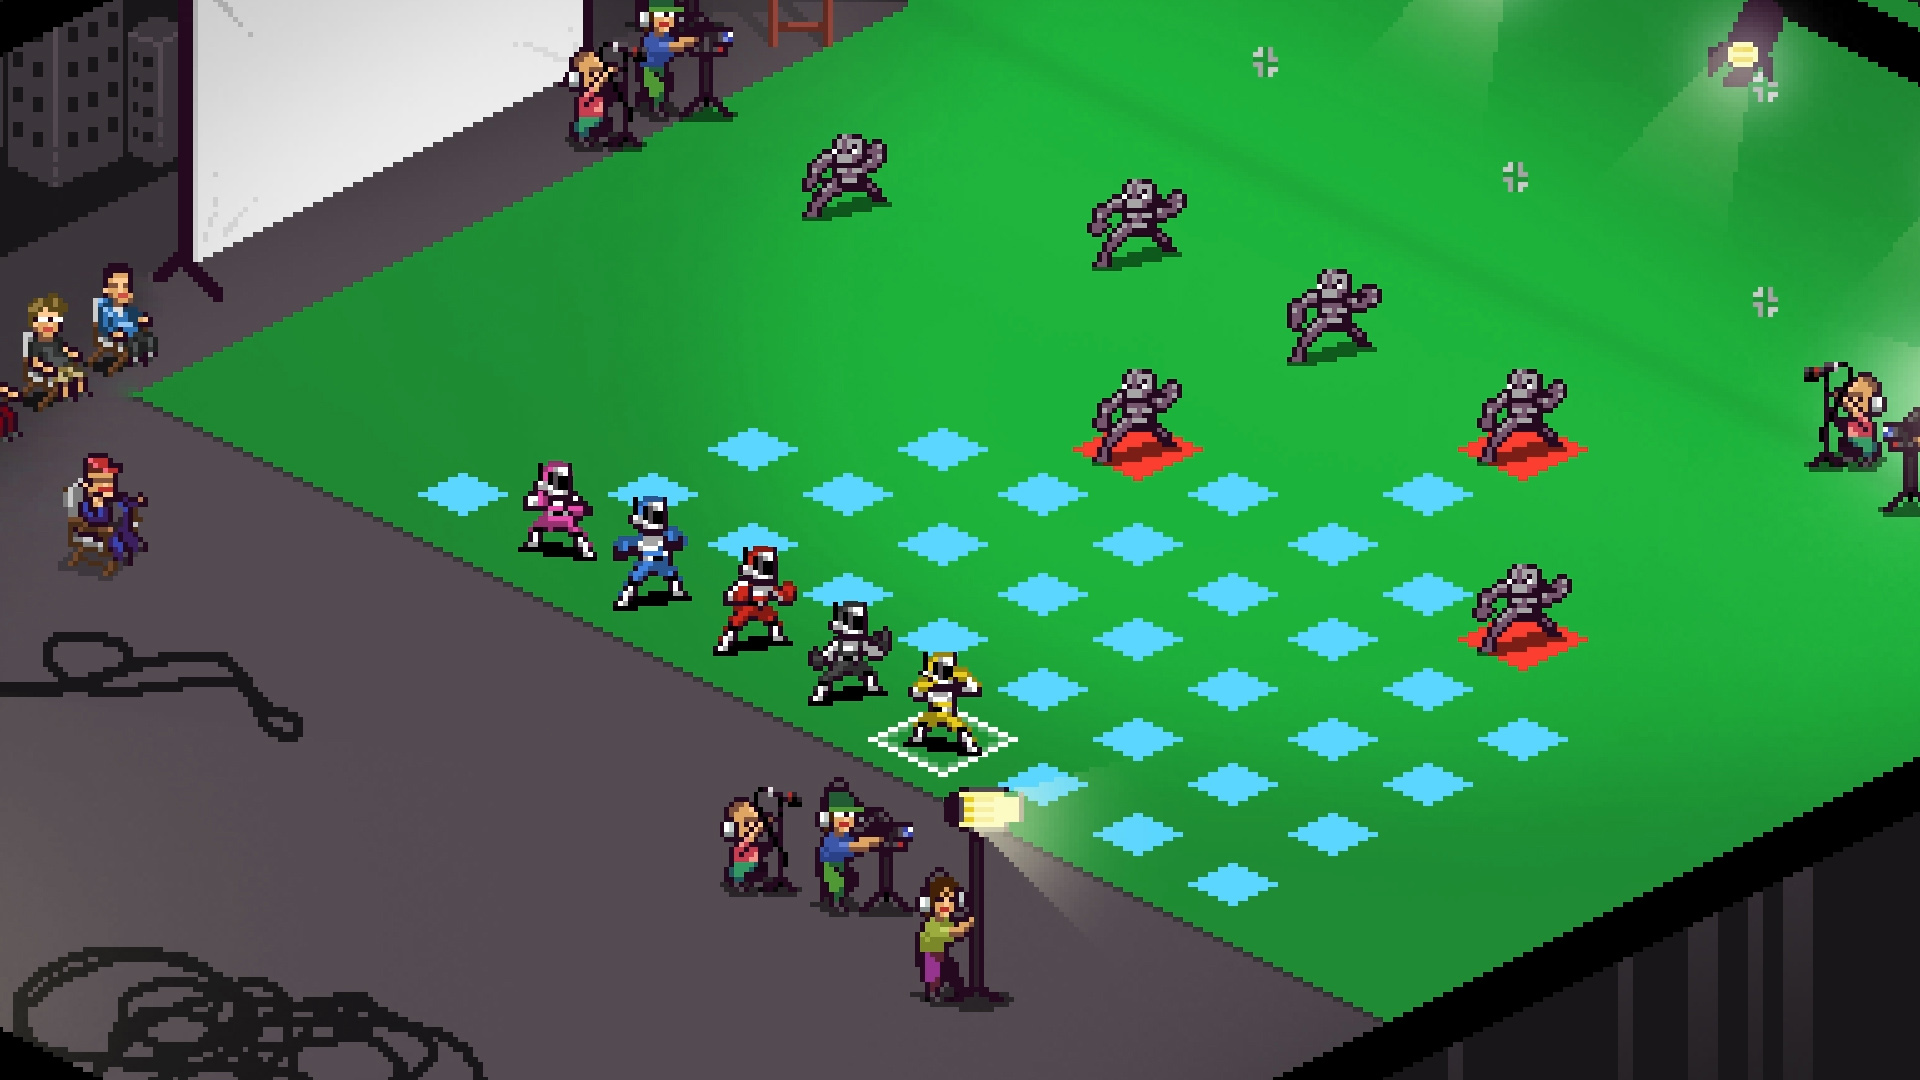
\includegraphics[width=0.8\textwidth]{figuras/Chroma Squad.jpg}
    \caption{Chroma Squad. Fonte: \cite{chromaSquad}}
    \label{fig:chroma-squad}
\end{figure}

\subsection{Dandara}
\textit{Dandara} é um jogo de ação e aventura desenvolvido pela Long Hat House, lançado em 2018 para múltiplas plataformas. O jogo apresenta uma jogabilidade única, baseada em movimentos de plataforma e combate, combinada com uma narrativa inspirada na cultura e história brasileira.

\textit{Dandara} é um exemplo de jogo brasileiro que se destaca pela qualidade de sua produção e pela originalidade de sua proposta. A estética visual e sonora do jogo, inspirada na cultura afro-brasileira, e a jogabilidade inovadora, que desafia os padrões do gênero, conquistaram a crítica e o público, tornando-se um dos títulos mais aclamados da Long Hat House.

\begin{figure}[H]
    \centering
    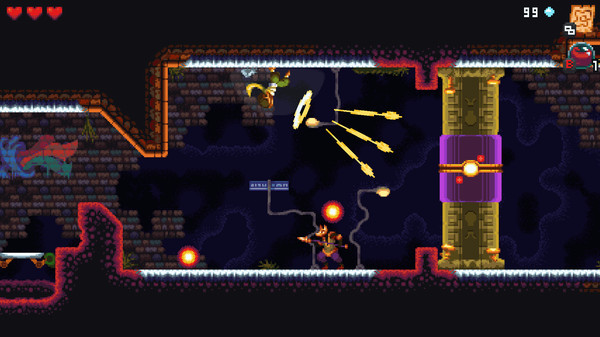
\includegraphics[width=0.8\textwidth]{figuras/Dandara.jpg}
    \caption{Dandara. Fonte: \cite{dandara}}
    \label{fig:dandara}
\end{figure}

\subsection{Aritana e a Pena da Harpia}
\textit{Aritana e a Pena da Harpia} é um jogo de ação e aventura desenvolvido pela Duaik Entertainment, lançado em 2014 para múltiplas plataformas. O jogo apresenta uma narrativa inspirada na mitologia indígena brasileira, combinada com uma jogabilidade baseada em movimentos de plataforma e combate.

\textit{Aritana e a Pena da Harpia} é um exemplo de jogo brasileiro que se destaca pela originalidade de sua proposta e pela qualidade de sua produção. A estética visual e sonora do jogo, inspirada na cultura indígena brasileira, e a narrativa envolvente, que explora temas como amizade, coragem e respeito à natureza, conquistaram a crítica e o público, tornando-se um dos títulos mais populares da Duaik Entertainment.

\begin{figure}[H]
    \centering
    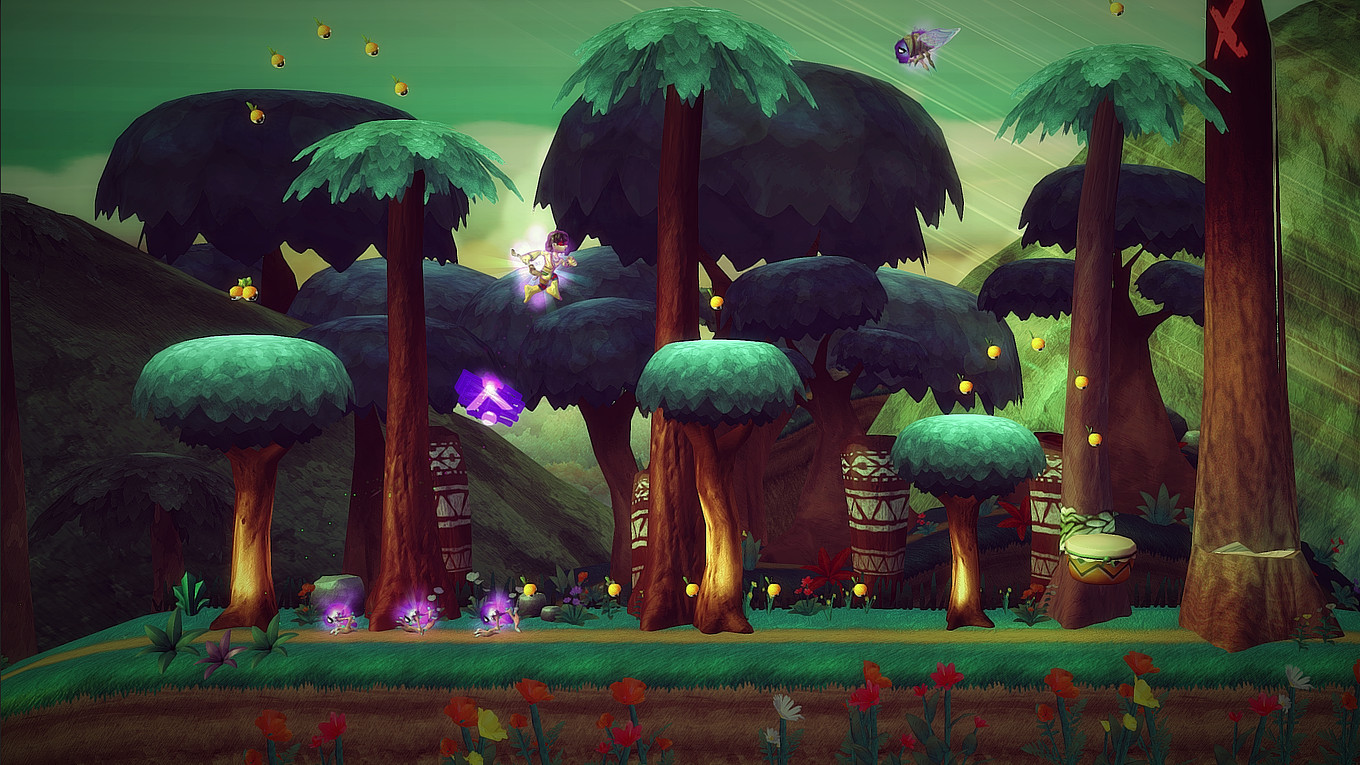
\includegraphics[width=0.8\textwidth]{figuras/Aritana.jpg}
    \caption{Aritana e a Pena da Harpia. Fonte: \cite{aritana}}
    \label{fig:aritana}
\end{figure}
\chapter{Escolha do jogo}

Para a escolha do jogo foi pensado em suprir a falta de jogos de corrida no mercado brasileiro, visto que o Brasil não possui muitos jogos de corrida, e os que existem são de empresas estrangeiras. Além disso, outros alunos do curso de Ciência da Computação da USP já haviam desenvolvido jogos em OpenGL onde foi possível, com o passar do tempo, aprimorar o conhecimento e a experiência com a biblioteca.

Com o uso do OpenGL e a utilização de memória gráfica, foi possível desenvolver um jogo de corrida em 3D, rápido e dinâmico, com a possibilidade de adicionar novos elementos e funcionalidades ao jogo.

\section{Gênero do jogo}

Além de tudo isso, por uma questão de preferência pessoal, foi escolhido um estilo de jogo que é muito popular e de grande apreço pelo autor, o estilo de corrida de Kart.

Vários jogos de corrida de Kart já foram desenvolvidos, como \textit{Mario Kart}, \textit{Crash Team Racing}, \textit{Blur}, \textit{Rock \& Roll Racing} entre vários outros. Todos esses jogos possuem características únicas e são muito divertidos de jogar, o que torna o gênero de corrida de Kart muito popular e apreciado por muitos jogadores.

\subsection{Mario Kart}

\textit{Mario Kart} é uma série de jogos de corrida de Kart desenvolvida e publicada pela Nintendo. O primeiro jogo da série foi lançado em 1992 para o Super Nintendo Entertainment System (SNES) e desde então a série se tornou uma das mais populares e bem-sucedidas da Nintendo.

Os jogos da série \textit{Mario Kart} são conhecidos por sua jogabilidade acessível e dinâmica, que combina elementos de corrida e combate, e por seus personagens carismáticos e coloridos, como Mario, Luigi, Peach, Bowser, Donkey Kong, Yoshi, entre outros.

\begin{figure}[H]
    \centering
    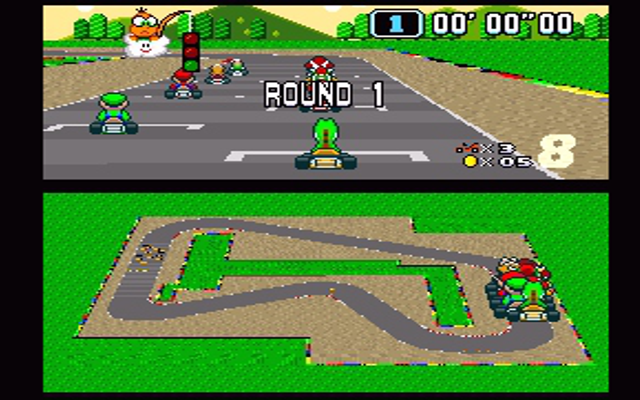
\includegraphics[width=0.8\textwidth]{figuras/Mario Kart.png}
    \caption{Mario Kart. \cite{marioKart}}
    \label{fig:mario-kart}
\end{figure}

\subsection{Crash Team Racing}

\textit{Crash Team Racing} é um jogo de corrida de Kart desenvolvido pela Naughty Dog e publicado pela Sony Computer Entertainment para o PlayStation em 1999. O jogo é conhecido por sua jogabilidade desafiadora e por seus personagens carismáticos, como Crash Bandicoot, Dr. Neo Cortex, Coco Bandicoot, entre outros.

\begin{figure}[H]
    \centering
    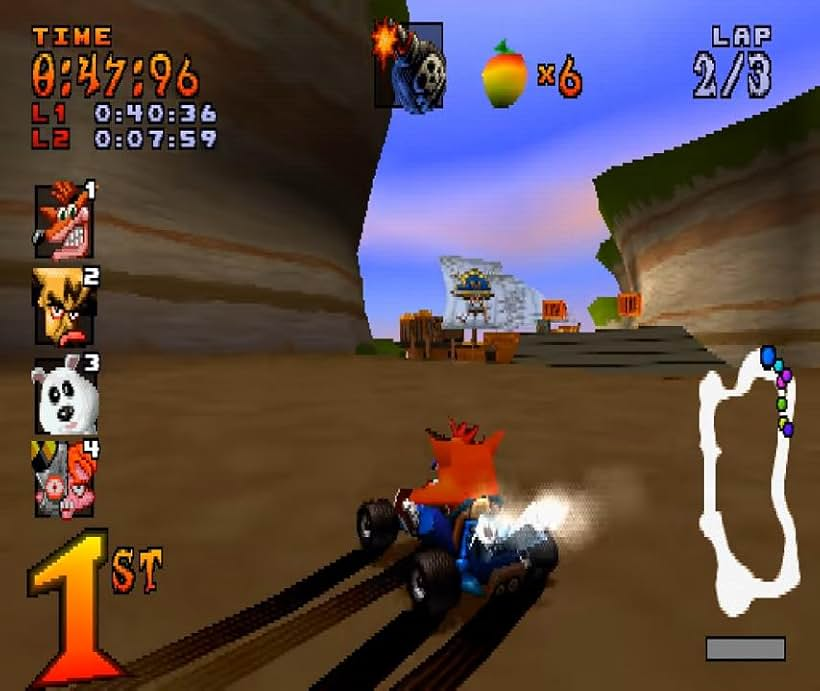
\includegraphics[width=0.8\textwidth]{figuras/Crash Team Racing.jpg}
    \caption{Crash Team Racing. \cite{crashTeamRacing}}
    \label{fig:crash-team-racing}
\end{figure}

Um de seus principais diferenciais é o modo de jogo \textit{Adventure}, onde o jogador deve competir em várias pistas e desafios para coletar cristais e chaves e derrotar Nitros Oxide, o vilão do jogo.

\textit{Crash Team Racing} foi um grande sucesso de crítica e público e se tornou um dos jogos de corrida de Kart mais populares do PlayStation, com milhões de cópias vendidas em todo o mundo.

Em 2019, a Activision lançou um remake do jogo, chamado \textit{Crash Team Racing Nitro-Fueled}, para PlayStation 4, Xbox One, Nintendo Switch e PC, que foi muito bem recebido pela crítica e pelos fãs da série, o que mostra o quanto o estilo de jogo é relevante e popular até hoje.

\begin{figure}[H]
    \centering
    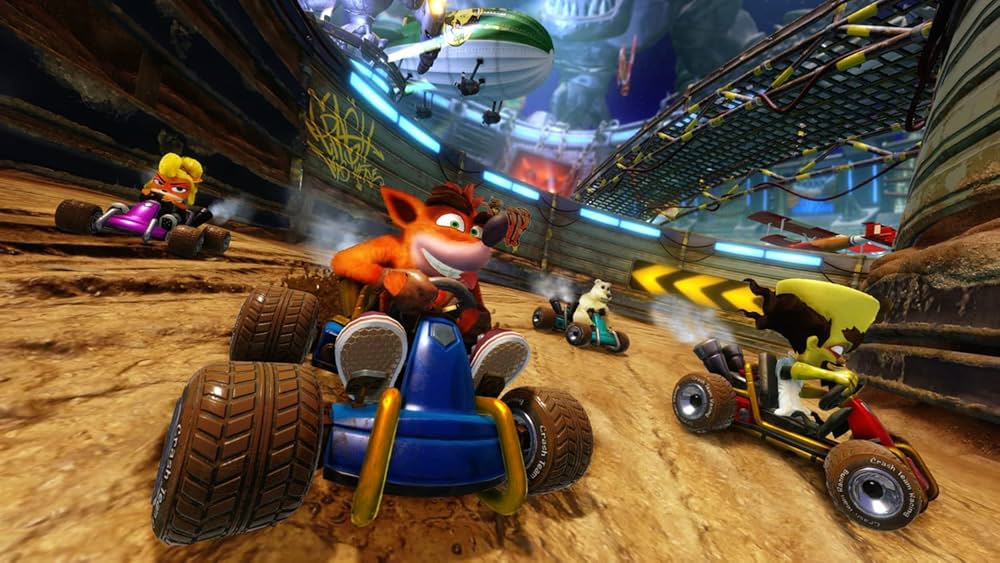
\includegraphics[width=0.8\textwidth]{figuras/Crash Team Racing Nitro Fueled.jpg}
    \caption{Crash Team Racing Nitro-Fueled. \cite{crashTeamRacingNitroFueled}}
    \label{fig:crash-team-racing-nitro-fueled}
\end{figure}

\subsection{Blur}

\textit{Blur} é um jogo de corrida de Kart desenvolvido pela Bizarre Creations e publicado pela Activision para PlayStation 3, Xbox 360 e PC em 2010. O jogo é conhecido por sua jogabilidade arcade e por seus gráficos realistas, que combinam elementos de corrida e combate.

Seu principal diferencial é o seu combate veicular, onde os jogadores podem usar power-ups para atacar e defender seus oponentes, como mísseis, minas, escudos, entre outros.

Nesse estilo de jogo, o jogador pode escolher entre vários carros e pilotos, cada um com suas próprias habilidades e características únicas, e competir em várias pistas e modos de jogo, como o modo carreira, modo de múltiplos jogadores, entre outros.

Ele não é tão semelhante aos jogos de corrida de Kart tradicionais, mas é um jogo muito divertido e desafiador, que combina elementos de corrida e combate de uma forma única e inovadora, com um tema mais adulto e realista.

\begin{figure}[H]
    \centering
    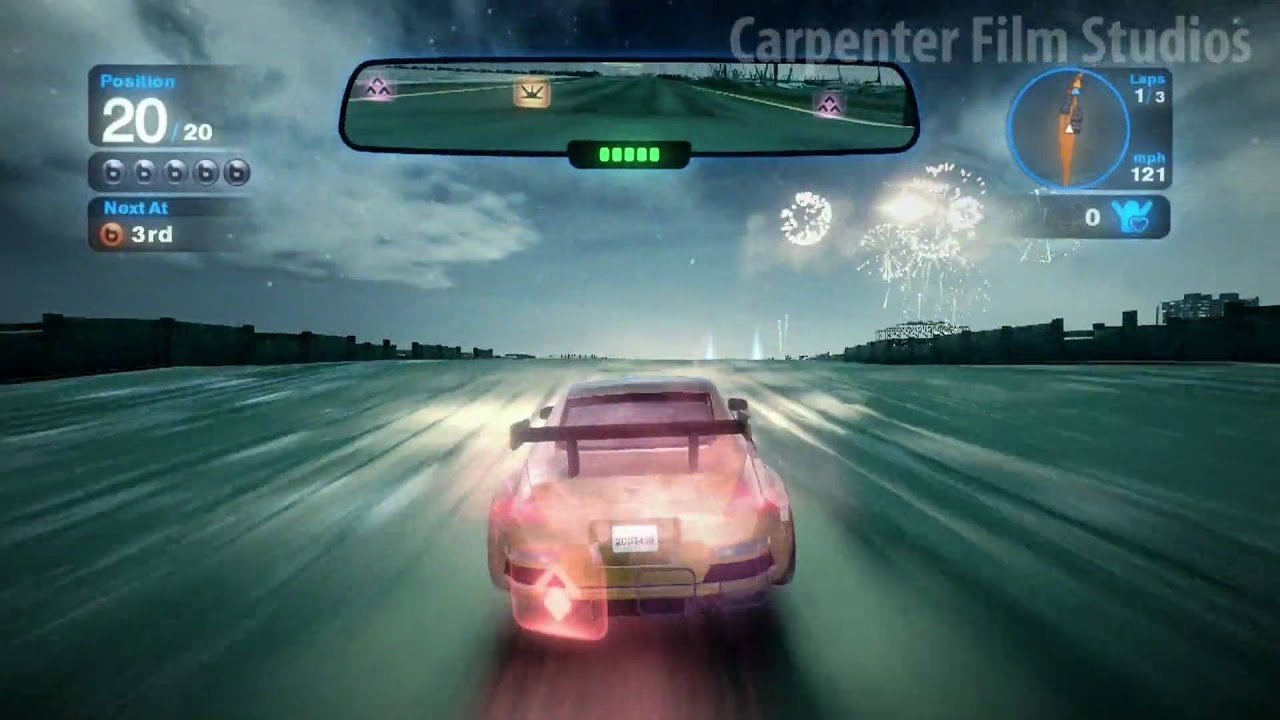
\includegraphics[width=0.8\textwidth]{figuras/Blur.jpg}
    \caption{Blur. \cite{blur}}
    \label{fig:blur}
\end{figure}

\subsection{Rock \& Roll Racing}

\textit{Rock \& Roll Racing} é um jogo de corrida de Kart desenvolvido pela Silicon \& Synapse (atual Blizzard Entertainment) e publicado pela Interplay Productions para o Super Nintendo Entertainment System (SNES) e Mega Drive em 1993.

O jogo é conhecido por sua jogabilidade acessível e dinâmica, que combina elementos de corrida e combate, e por sua trilha sonora de \textit{rock and roll}, que inclui músicas de bandas como Black Sabbath, Deep Purple, Steppenwolf, entre outras.

A ideia do jogo é envolver o jogador numa corrida de Kart futurista, onde ele deve competir em várias pistas e desafios para ganhar dinheiro e comprar novos carros e armas, que podem ser usados para atacar e defender seus oponentes.

Diferente dos outros jogos de corrida de Kart, \textit{Rock \& Roll Racing} é um jogo de corrida de Kart isométrico, onde o jogador vê o carro de cima, o que dá uma perspectiva diferente e única ao jogo.

\begin{figure}[H]
    \centering
    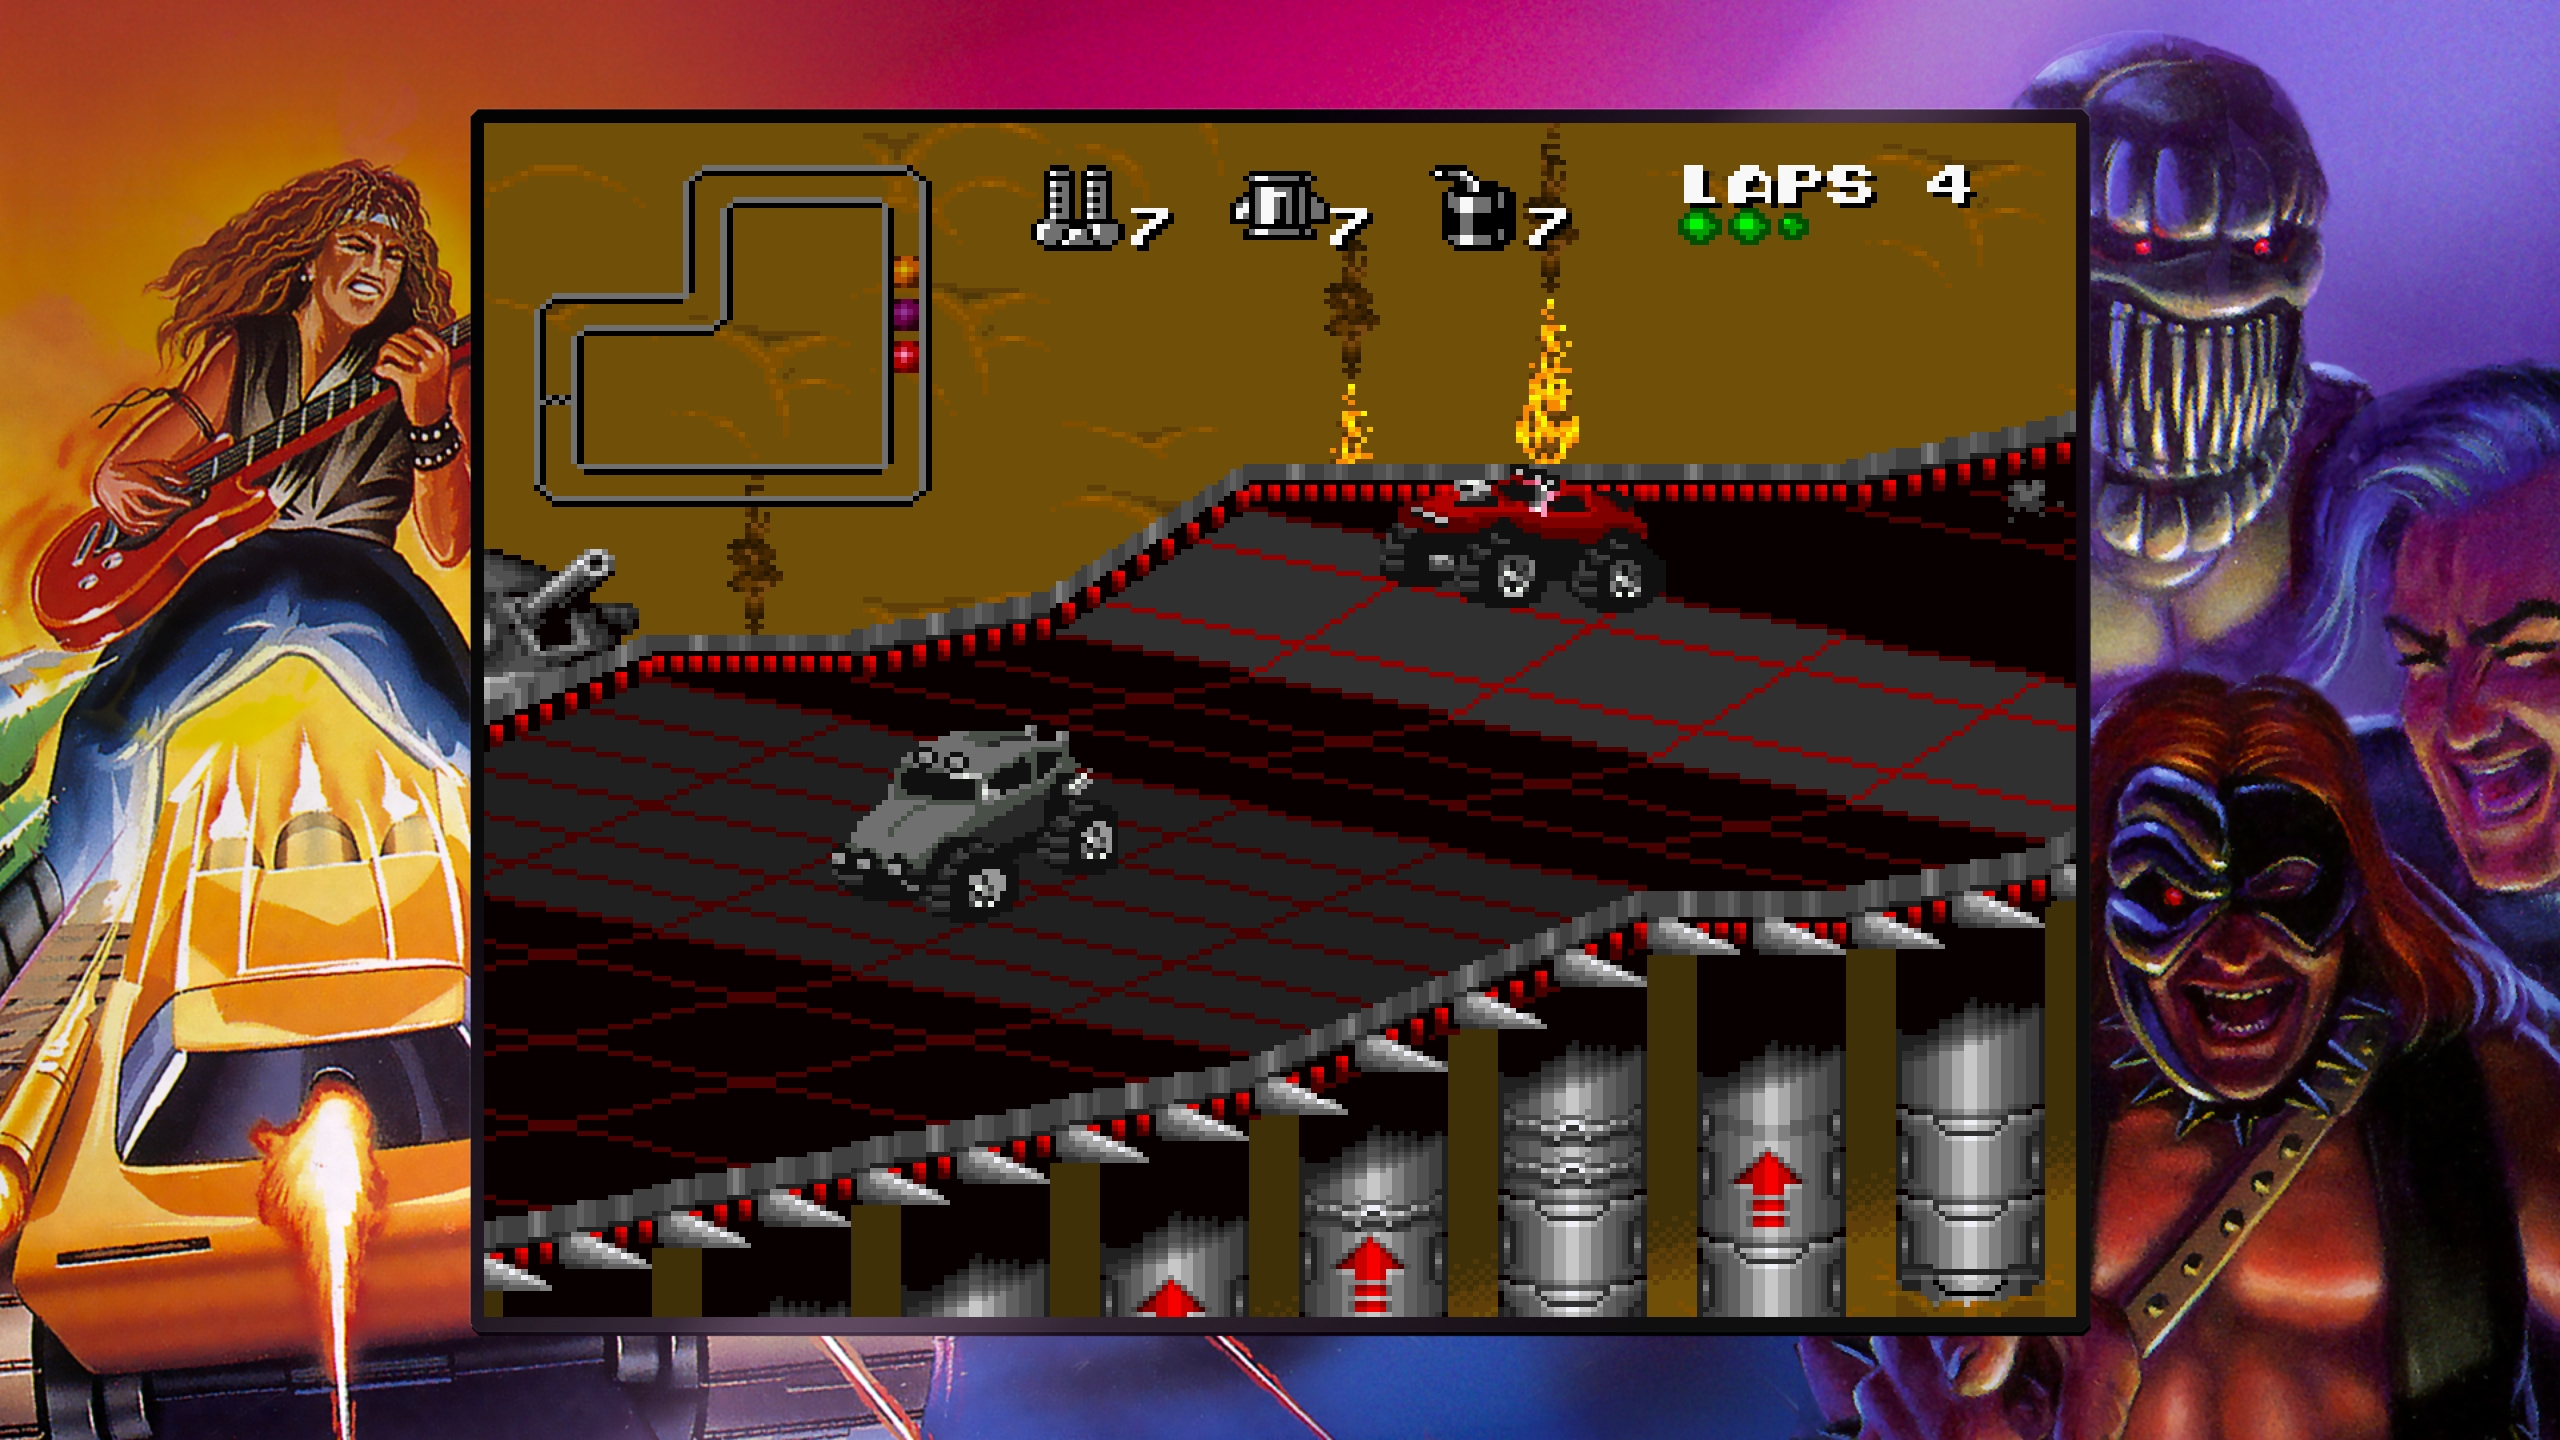
\includegraphics[width=0.8\textwidth]{figuras/Rock and Roll Racing.jpg}
    \caption{Rock \& Roll Racing. \cite{rockAndRollRacing}}
    \label{fig:rock-and-roll-racing}
\end{figure}

\section{Influência do gênero no mercado}

O gênero de corrida de Kart é muito popular e apreciado por muitos jogadores, de todas as idades e gêneros, e é um dos gêneros mais bem-sucedidos e lucrativos da indústria de jogos eletrônicos. Vários jogos de corrida de Kart já foram desenvolvidos e lançados para diferentes plataformas, como o SNES, PlayStation, Xbox, PC, entre outros, e muitos deles se tornaram grandes sucessos de crítica e público.

Além disso, o gênero de corrida de Kart é muito versátil e diversificado, o que permite a criação de jogos com diferentes estilos e mecânicas de jogo, que podem atrair diferentes categorias de jogadores e públicos. Por exemplo, \textit{Mario Kart} é conhecido por sua jogabilidade acessível e dinâmica, que combina elementos de corrida e combate, e por seus personagens carismáticos e coloridos, como Mario, Luigi, Peach, Bowser, Donkey Kong, Yoshi, entre outros.

\subsection{Sucesso financeiro}

A franquia \textit{Mario Kart} é uma das mais bem-sucedidas da Nintendo, com milhões de cópias vendidas em todo o mundo e vários jogos lançados para diferentes plataformas, como o SNES, Nintendo 64, GameCube, Wii, Wii U, Nintendo DS, Nintendo 3DS, Nintendo Switch, entre outros.

Hoje em dia, \textit{Mario Kart 8 Deluxe} é o jogo de corrida de Kart mais vendido de todos os tempos, com mais de 70.43 milhões de cópias vendidas em todo o mundo. A série \textit{Mario Kart} não só foi popular entre os jogos de corrida, já que além de ser o jogo mais vendido para o\textit{Nintendo Switch}, console da Nintendo, também é o sexto jogo mais vendido de todos os tempos, considerando todas as plataformas e gêneros (\cite{bestSellingGames}).

\begin{figure}[H]
    \centering
    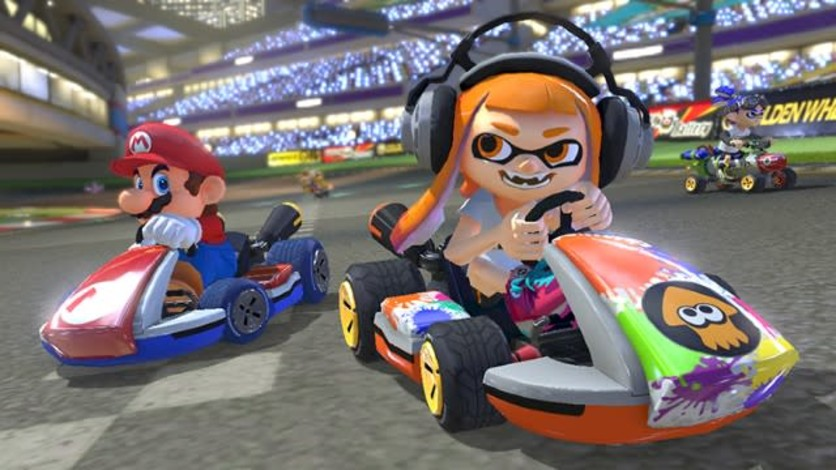
\includegraphics[width=0.8\textwidth]{figuras/Mario Kart 8.jpg}
    \caption{Mario Kart 8 Deluxe. \cite{marioKart8}}
    \label{fig:mario-kart-8-deluxe}
\end{figure}

\subsection{Impacto social}

O gênero inteiro de corrida de Kart é muito popular e apreciado por muitos jogadores, de todas as idades e gêneros, e é também tão importante que influenciou a cultura pop e a sociedade de várias maneiras.

Em uma pesquisa feita pela \textit{BonusFinder}, foi descoberto que \textit{Mario Kart} não é somente o jogo de corrida mais popular, mas também é o terceiro jogo mais estressante de todos os tempos. A pesquisa foi medindo o aumento da frequência cardíaca dos jogadores enquanto jogavam, e \textit{Mario Kart} aumentou a frequência cardíaca em 73.44\% (\cite{stressful:bonusFinder}). Isso mostra o quanto o jogo é popular e apreciado por muitos jogadores, de todas as idades e gêneros, e o quanto ele é importante para a cultura pop e a sociedade.
\chapter{Escolha dos gráficos}

Jogos estilo \textit{Kart} são conhecidos por sua jogabilidade acessível e dinâmica, que combina elementos de corrida e combate, e por seus personagens carismáticos e coloridos. No gênero temos vários estilos visuais a serem explorados, desde gráficos 2D até gráficos 3D realistas.

\section{Jogos 2D (ou 2.5D)}

O primeiro \textit{Mario Kart} foi lançado em 1992 para o Super Nintendo Entertainment System (SNES) e desde então a série se tornou uma das mais populares e bem-sucedidas da Nintendo. O jogo foi desenvolvido em 2D, principalmente por limitações técnicas da época, mas o jogo realiza uma simulação de 3D, com artes em 2D que se movem em um ambiente 3D simulado, o que é conhecido como gráficos 2.5D.

\subsection{Gráficos e lógica bidimensional}

Esse estilo de gráficos foi muito explorado na época dos consoles de 16 bits, como o SNES e o Mega Drive, e ainda é muito popular em jogos \textit{indie} e \textit{mobile}, devido à sua simplicidade e facilidade de desenvolvimento. Além disso, esse estilo de gráficos é muito charmoso e nostálgico, o que atrai muitos jogadores, por isso é uma ótima opção para jogos de Kart (\cite{graficos2.5D}). Para uma melhor compreensão, veja a Figura \ref{fig:mario-kart}.

Podemos explicar este estilo 2.5D como um jogo 2D que simula um ambiente 3D, com personagens e cenários em 2D, mas com movimentação e câmera simulando um ambiente 3D. Isso é feito através de técnicas de renderização e animação, que dão a ilusão de profundidade e movimento tridimensional.

\subsection{Implementação moderna, lógica 2D e gráficos 3D}

Hoje em dia não temos tal limitação técnica, mas o estilo 2.5D ainda é muito popular, principalmente em jogos indie e mobile, devido à sua simplicidade e facilidade de desenvolvimento. Isso facilita a produção de jogos com gráficos bonitos e charmosos, porém com uma lógica que só considera um espaço bidimensional, o que simplifica o desenvolvimento e a programação.

Um exemplo de um jogo onde se usa esse estilo de gráficos é o \textit{Mario Wonder} (\cite{marioWonder}), recente e tem toda a sua lógica programada em um espaço limitado 2D, porém sua aparência visual é completamente processada em 3D.

\begin{figure}[H]
    \centering
    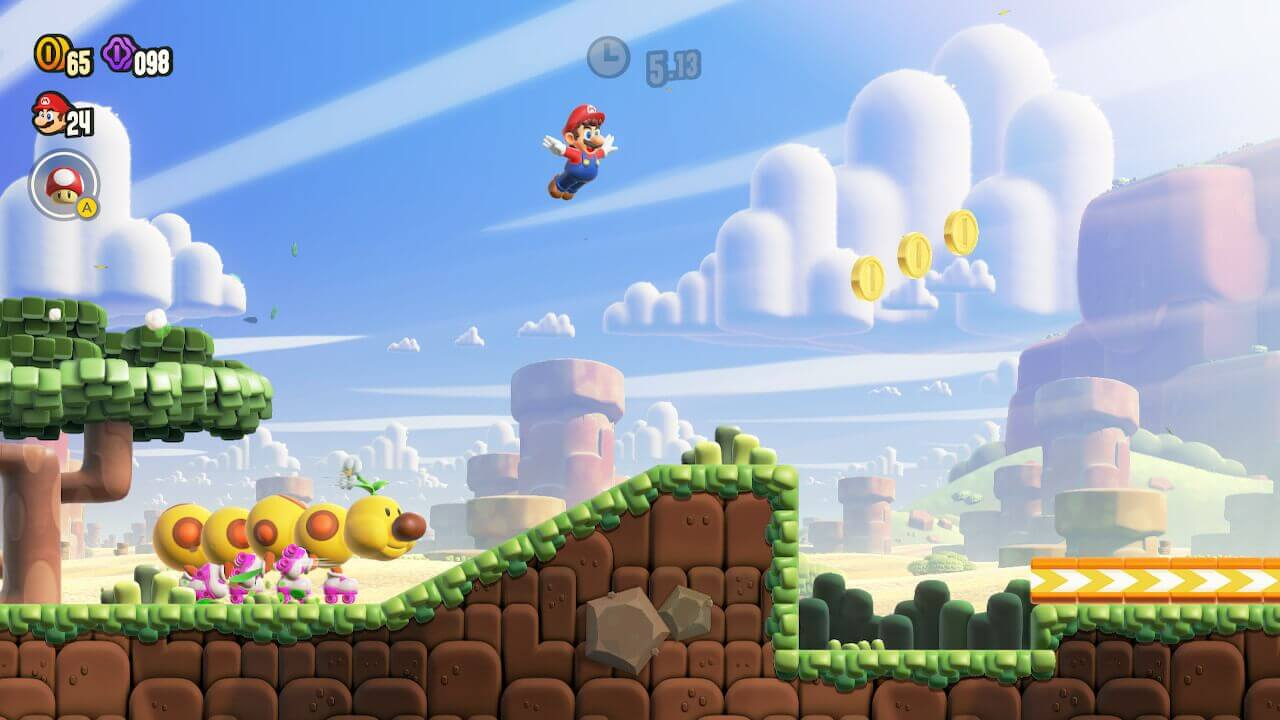
\includegraphics[width=0.8\textwidth]{figuras/Mario Wonder.jpg}
    \caption{Mario Wonder. \cite{marioWonder}}
    \label{fig:mario-wonder}
\end{figure}

\section{Jogos 3D}

Outra opção seria desenvolver o jogo totalmente em 3D, com gráficos realistas e ambientes tridimensionais, o que daria uma sensação de imersão e realismo muito maior, mas também seria muito mais complexo e demorado de desenvolver. Além disso, o estilo 3D é mais comum em jogos de corrida de Kart mais recentes, como \textit{Crash Team Racing Nitro-Fueled} e \textit{Blur}, que possuem gráficos realistas e ambientes tridimensionais, com texturas e efeitos visuais muito bem detalhados.

Para isso devemos pensar num ambiente tridimensional na totalidade, não somente quanto à parte visual, mas também com a lógica do jogo, que deve considerar um espaço tridimensional, com movimentação e colisão em três dimensões. Isso é muito mais complexo e demorado de desenvolver, mas o resultado é muito mais imersivo e realista, o que pode atrair mais jogadores e fãs do gênero.

\section{Decisão}

Optamos pelo desenvolvimento do \textit{USP Kart} em 2.5D, lógica bidimensional, mas com gráficos 3D, utilizando do OpenGL moderno para renderização e animação, o que gera uma sensação de profundidade e movimento tridimensional, mas com uma lógica simplificada e mais fácil de desenvolver. Isso viabilizou a produção do jogo, permitindo seu desenvolvimento de maneira compatível com a duração de um trabalho de conclusão de curso.
\chapter{USP Kart}

O objetivo deste trabalho foi o desenvolvimento do jogo \textit{USP Kart}, um jogo de corrida estilo \textit{Kart} com temática da Universidade de São Paulo (USP). O jogo foi desenvolvido em C++ com OpenGL moderno e tem como principal característica a corrida com karts em um ambiente universitário, com personagens inspirados na mascote Fluffy.

Para isso foi escolhido uma lógica bidimensional, porém com gráficos tridimensionais, o que facilitou o desenvolvimento e permitiu que o jogo fosse lançado mais rapidamente. O jogo foi desenvolvido em duas máquinas, uma com Windows e outra com Linux, ou seja, tudo o que foi desenvolvido deve ser compatível com ambos os sistemas operacionais.

\section{Estilo artístico}

Como mencionado anteriormente, o jogo visa retratar uma corrida de karts em um ambiente universitário, dessa forma não utilizado modelos externos, mas a arte em geral foi desenvolvida pelos próprios desenvolvedores. A arte foi feita utilizando um programa de modelagem simples, o \textit{Blockbench}, que permite a criação de modelos 3D simples e com baixa quantidade de polígonos.

Com exceção do mapa, todos os modelos foram feitos no \textit{Blockbench}, e a textura foi feita no \textit{GIMP}, um editor de imagens gratuito e de código aberto. A textura foi feita de forma simples, com cores sólidas e sem muitos detalhes, para manter a simplicidade e a leveza do jogo.

\pagebreak

\section{Personagens}

Todos os personagens seguem o mesmo modelo, e mesma textura, porém o jogo contém uma lógica de substituição de cores, permitindo que eu filtre e substitua uma cor por outra, fazendo uma identificação única para cada personagem. Os personagens são inspirados na mascote Fluffy, e possuem uma textura simples, com cores sólidas e sem muitos detalhes.

\begin{figure}[H]
    \centering
    \begin{subfigure}[b]{1\textwidth}
        \centering
        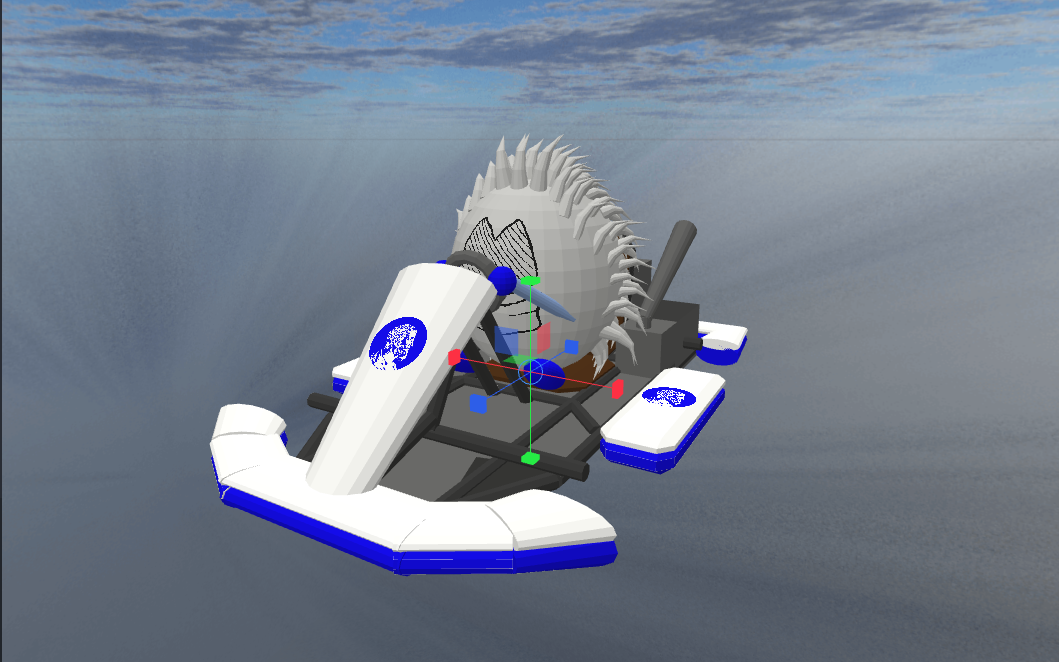
\includegraphics[width=0.8\textwidth]{figuras/Fluffy.png}
        \caption{Modelo do Fluffy no \textit{Blockbench}.}
        \label{fig:fluffy-blockbench}
    \end{subfigure}
    \begin{subfigure}[b]{1\textwidth}
        \centering
        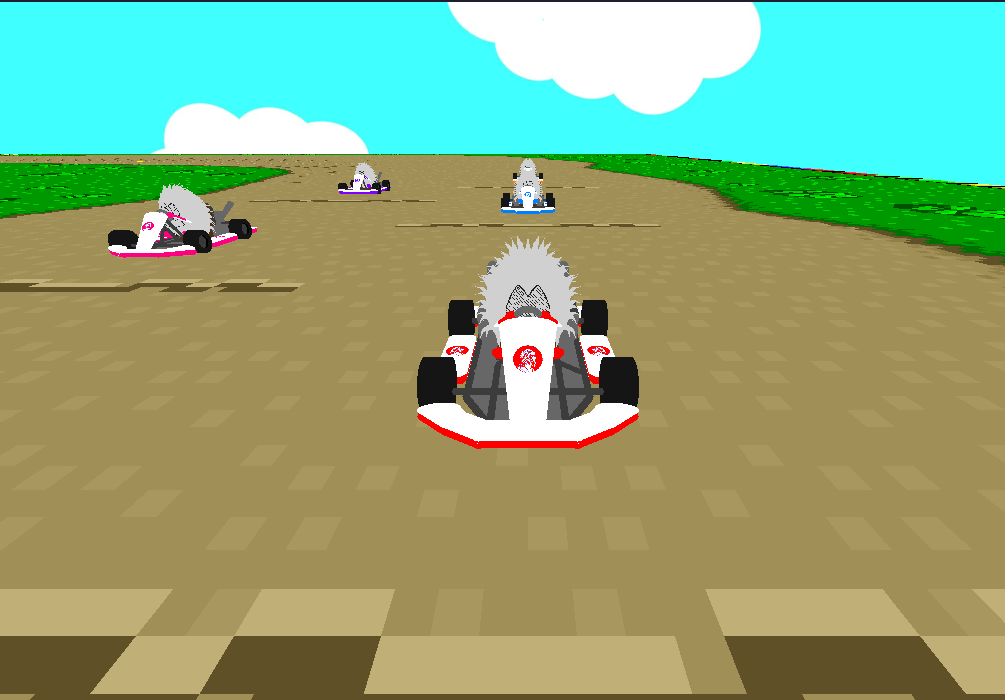
\includegraphics[width=0.8\textwidth]{figuras/USP Kart.png}
        \caption{Várias variantes do Fluffy com cores diferentes.}
        \label{fig:fluffy-variantes}
    \end{subfigure}
    \caption{Fluffy no USP Kart.}
    \label{fig:fluffy}
\end{figure}

\section{Mapa}

O mapa é completamente em 2D, basicamente uma textura sólida com um caminho desenhado, ele não foi criado pelo desenvolvedor, mas teve de ser adaptado para o jogo. Esse mapa em específico se chama \textit{Donut Plains 1}, do \textit{Mario Kart} (\cite{marioKart}). O mapa é composto por um caminho principal e alguns atalhos, que podem ser utilizados para ganhar vantagem na corrida. Os atalhos são sutis e podem custar tempo se não forem utilizados corretamente.

\begin{figure}[H]
    \centering
    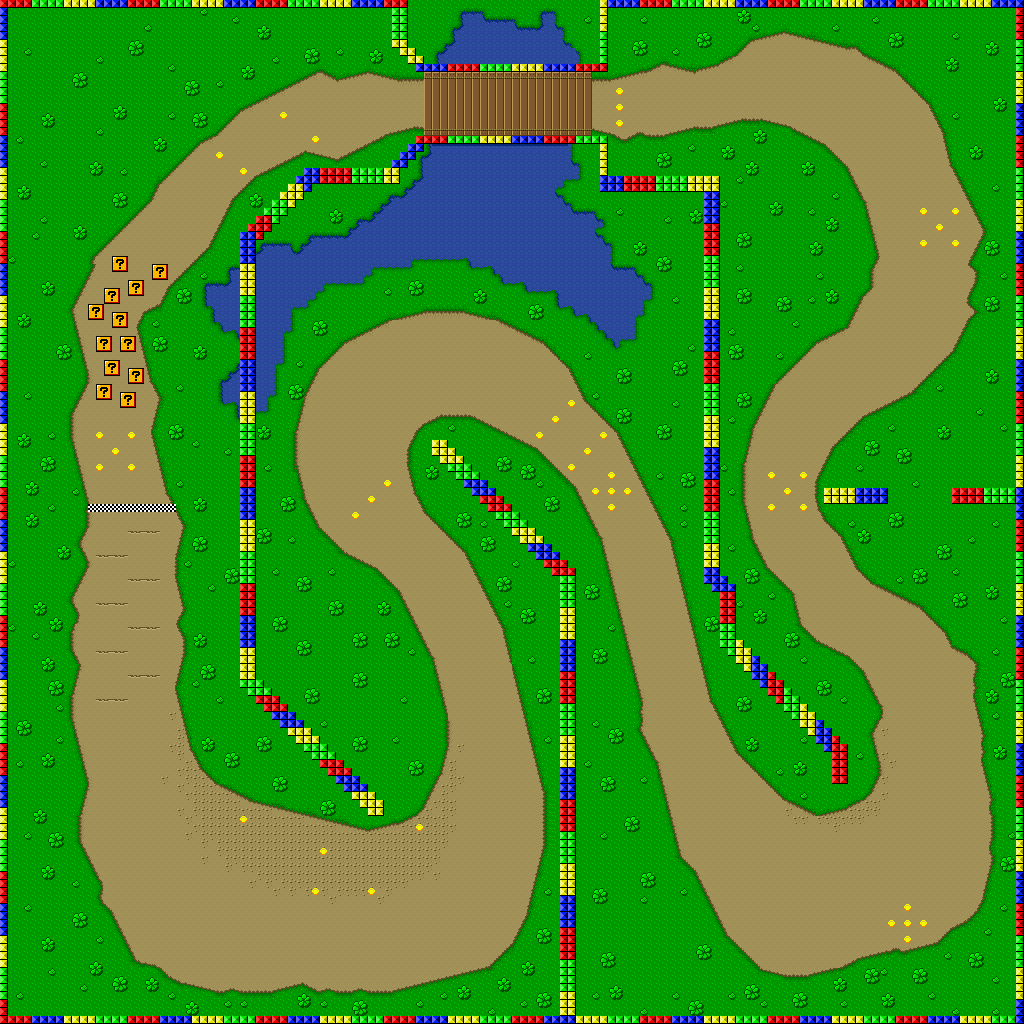
\includegraphics[width=0.8\textwidth]{figuras/Mapa.png}
    \caption{Mapa utilizado no USP Kart, Donut Plains 1. \cite{marioKart}}
    \label{fig:mapa}
\end{figure}


No mapa temos vários pontos de controle, apesar de invisíveis ao jogador, eles são utilizados para verificar se o jogador está no caminho correto, e caso não esteja, ele é incapaz de prosseguir. Os pontos de controle são extensos e poucos em quantidade, porém são o suficiente para garantir que o jogador esteja no caminho correto e não esteja trapaceando.

Também é válido notar que, com exceção do ponto de partida, todos os pontos de controle são o mais extensos o possível, fazendo com que o jogador possa passar por eles de qualquer direção, desde que esteja progredindo e se aproximando da linha de chegada.

\section{Jogabilidade}

O jogo foi pensado para ser o mais responsivo o possível, utilizando do padrão de projeto \textit{State}, o personagem não realiza nenhuma ação além de mudar o seu estado, fazendo com que a transição de movimento seja muito mais suave e natural. O jogo também possui um sistema de colisão simples, mas eficaz, que permite que o personagem colida com objetos e outros personagens.

O jogador não possui nenhuma ação além de acelerar, frear e virar, o que simplifica a jogabilidade e permite que o jogador se concentre na corrida. Essas mesmas ações são utilizadas para todos os personagens, controlados pelo jogador ou não, fazendo com que as corridas sejam justas e equilibradas. O nome dessa técnica é \textit{rubber banding} (\cite{rubberBandAi}), que é uma técnica utilizada em jogos de corrida para manter a competição acirrada, mesmo que o jogador esteja muito à frente ou muito atrás dos outros.

Apesar disso, caso o jogador esteja muito atrás dos outros, os personagens controlados pela inteligência artificial (IA) diminuem a velocidade, permitindo que o jogador possa alcançá-los e ultrapassá-los. O contrário também acontece, caso o jogador esteja muito à frente, os personagens controlados pela IA aumentam a velocidade, permitindo que o jogador possa ser ultrapassado.

\section{Interface gráfica}

Apesar das bibliotecas utilizadas terem ajudado bastante no desenvolvimento do jogo, a interface gráfica se mostrou um grande desafio e é extremamente básica, consistindo de um texto no canto superior esquerdo da tela, que mostra a posição do jogador e a quantidade de quadros por segundo sendo desenhados, e um texto no canto superior direito da tela, que mostra a quantidade de voltas completadas.
\chapter{Desenvolvimento do USP Kart}

No desenvolvimento do USP Kart, foram utilizadas diversas ferramentas e tecnologias para a implementação de um jogo de corrida estilo \textit{Kart} em 2.5D, com gráficos 3D e lógica bidimensional. Neste capítulo, serão apresentadas as principais ferramentas e tecnologias utilizadas, bem como a implementação de cada uma delas.

Primeiramente é necessário destacar que para que tudo fosse implementado foram necessários mais de uma categoria de padrão de projeto, como o \textit{Singleton}, por exemplo, este sendo o mais citado pelos gerenciadores e controladores de recursos, para serem acessados de qualquer lugar do código.

Também é importante destacar que o desenvolvimento do jogo foi feito em C++, utilizando de diversas bibliotecas e \textit{frameworks} para a implementação de cada parte do jogo, como o OpenGL para a renderização dos gráficos, o OpenAL para a reprodução de áudios, o Assimp para a importação de modelos 3D, entre outros.

Já que a linguagem C++ foi escolhida foi utilizado de paralelismo para a execução de várias tarefas, em destaque a separação da lógica do jogo e a renderização dos gráficos, para que o jogo possa ser o mais otimizado possível.

\section{Ferramentas desenvolvidas}

Como o jogo não possui um motor de jogo, foi necessário implementar diversas ferramentas e sistemas para ser desenvolvido. Dentre as principais estão o gerenciador de recursos, o gerenciador de configurações gráficas, o registrador de mensagens, o sistema gráfico e a classe de dados.

\subsection{Gerenciador de recursos}

O gerenciador de recursos foi implementado principalmente para garantir que todos os recursos fossem carregados e processados uma única vez, ou seja, um modelo em 3D de um kart não seria carregado mais de uma vez, evitando assim a duplicação de dados e economizando memória. Para isso, o gerenciador de recursos foi implementado com o padrão de projeto \textit{Singleton}, para que possa ser acessado de qualquer lugar do código e garantir que somente uma instância seja criada.

O funcionamento disso se dá através de um \textit{map} que armazena todos os recursos carregados, e ao requisitar um recurso, o gerenciador verifica se ele já foi carregado, e caso não tenha sido, ele é carregado e armazenado no \textit{map}.

\subsubsection{Texturas}

As texturas são um dos recursos carregados pelo gerenciador. Para implementar essa lógica foi criado uma classe \textit{Texture} que armazena o ID da textura, o caminho do arquivo, tipo da textura, tamanho, quantidade de canais e o dado bruto (utilizado somente pelo OpenGL).

\subsubsection{Ícones}

Também no gerenciador de recursos foi implementado o carregamento de ícones, apesar de não ser tão necessário, pois não é preciso carregar mais de uma vez, foi implementado para manter a consistência do código, uma vez tão semelhante ao carregamento de texturas.

Apesar da semelhança vale lembrar que os ícones são mais simples que texturas, é salvo somente seus dados brutos, mas mesmo assim, também para garantir uma boa organização, facilitando não só o armazenamento dos dados, mas a consistência entre diferentes plataformas. 

Já que o USP Kart foi desenvolvido em duas máquinas, uma com Windows e outra com Linux, foi necessário tratar diferentemente, principalmente por dificuldades com a lógica de ícones no \textit{Wayland}, servidor gráfico padrão do Linux.

\subsubsection{Modelos 3D}
\subsubsection{Áudios}

\subsection{Gerenciador de configurações gráficas}

\subsection{Registrador de mensagens}
\subsubsection{Fila}
\subsubsection{Escrita em arquivo}

\subsection{Sistema de interface gráfica}
\subsubsection{Fila}
\subsubsection{Texto}

\subsection{Classe de dados}

\section{Gráficos com OpenGL}
\subsection{Criação de janela}
\subsection{Shaders}
\subsection{Texturas}
\subsection{Modelos 3D}
\subsection{Skybox}
\subsection{Animação}

\section{Mapa}
\subsection{Modelagem do mapa}
\subsection{Controlador do mapa}
\subsection{Pontos de controle}

\section{Lógica por objetos}
\subsection{Modelos de objetos}
\subsection{Transformações}

\section{Modelagem dos karts}
\subsection{Bicycle model}
\subsection{Implementação das rodas}

\section{Física}
\subsection{Objetos estáticos}
\subsection{Objetos com física}

\subsection{Movimentação}
\subsubsection{Força}
\subsubsection{Aceleração}

\subsection{Colisão}
\subsubsection{Detecção de colisão}
\subsubsection{Resolução de colisão}

\subsection{Limitação com o mapa}

\section{Personagens}

\subsection{Jogador}
\subsubsection{Controles}

\subsection{Inteligência artificial}
\subsubsection{Visão do ambiental}
\subsubsection{Tomada de decisão}
\subsubsection{Modelo Elástico}
\chapter{Resultados}

O desenvolvimento do \textit{USP Kart} foi concluído com sucesso, resultando em um jogo de corrida estilo \textit{Kart} com temática da Universidade de São Paulo (USP). Foi desenvolvido em C++ com OpenGL moderno e tem como principal característica a corrida com karts em um ambiente universitário, com personagens inspirados na mascote Fluffy.

O jogo foi desenvolvido em duas máquinas, uma com Windows 11 e outra com Fedora Linux 41 (Workstation), ou seja, tudo o que foi desenvolvido deve ser compatível com ambos os sistemas operacionais.

\section{Desempenho}

Percebe-se que o jogo tem algumas partes que devem ser otimizadas para rodar em computadores mais antigos, já que se utiliza de várias \textit{threads}, não é possível garantir que o jogo rode em computadores com poucos núcleos de processamento.

Os resultados obtidos foram uma utilização muito grande do processador e muito pequena da placa de vídeo, o que indica que o jogo é muito dependente do processador, e que a placa de vídeo não é utilizada eficientemente.

\section{Arte}

A arte do jogo ficou bem simples e não tão uniforme, já que foi elaborada por um desenvolvedor sem experiência em modelagem 3D. A textura dos personagens é simples, com cores sólidas e sem muitos detalhes, mas a escolha artística não foi tão satisfatória quanto o esperado, já que poucos modelos foram feitos concretamente, fazendo com que o jogo pareça inacabado.

\section{Jogabilidade}

O jogo tem excelente jogabilidade, com controles simples e bem responsivos, o que permite que o jogador se concentre na corrida. O sistema de colisão é simples, com certas falhas, mas eficaz, permitindo que o personagem colida com objetos e outros personagens.

O jogador não possui nenhuma ação além de acelerar, frear e virar, o que simplifica a jogabilidade e permite que o jogador se concentre na corrida. Essas mesmas ações são utilizadas para todos os personagens, controlados pelo jogador ou não, fazendo com que as corridas sejam justas e equilibradas.

Infelizmente a inteligência artificial não processa informações rápido o suficiente, fazendo com que o jogo pareça mais fácil do que deveria ser, já que os personagens controlados pelo computador dependem muito de um excelente desempenho no computador atualmente, o que não foi o caso com máquinas mais simples.

O jogo também não contou com habilidades especiais, o que poderia tornar o jogo mais interessante e desafiador, já que o jogador teria que aprender a utilizar essas habilidades especiais para vencer as corridas.

\section{Possíveis melhorias}

Como possíveis melhorias, pode-se citar a otimização do jogo para rodar em computadores mais antigos, a melhoria da arte, mais modelos, a adição de habilidades especiais para os personagens, para tornar o jogo mais interessante e desafiador, e a melhoria da inteligência artificial na totalidade.

\section{Testes e validação}

\textit{USP Kart} foi testado de maneira informal por 10 pessoas diferentes, com idades variadas, e todos os testadores gostaram do jogo, achando-o divertido, mas muito simples, o que indica que o jogo é bom, mas pode ser melhorado.

\section{Conclusão}

O desenvolvimento do \textit{USP Kart} foi concluído com sucesso, resultando em um jogo de corrida estilo \textit{Kart} com temática da Universidade de São Paulo (USP).

Apesar dos problemas encontrados, o jogo é divertido, com controles simples e responsivos. A arte é simples, mas eficaz, e a temática da USP é bem representada.




%%%%%%%%%%%%%%%%%%%%%%%%%%%% APÊNDICES E ANEXOS %%%%%%%%%%%%%%%%%%%%%%%%%%%%%%%%

% Um apêndice é algum conteúdo adicional de sua autoria que faz parte e
% colabora com a ideia geral do texto mas que, por alguma razão, não precisa
% fazer parte da sequência do discurso; por exemplo, a demonstração de um
% teorema intermediário, as perguntas usadas em uma pesquisa qualitativa etc.
%
% Um anexo é um documento que não faz parte da tese (em geral, nem é de sua
% autoria) mas é relevante para o conteúdo; por exemplo, a especificação do
% padrão técnico ou a legislação que o trabalho discute, um artigo de jornal
% apresentando a percepção do público sobre o tema da tese etc.
%
% Os comandos appendix e annex reiniciam a numeração de capítulos e passam
% a numerá-los com letras. "annex" não faz parte de nenhuma classe padrão,
% foi criado para este modelo. Se o trabalho não tiver apêndices ou anexos,
% remova estas linhas.
%
% Diferentemente de \mainmatter, \backmatter etc., \appendix e \annex não
% forçam o início de uma nova página. Em geral isso não é importante, pois
% o comando seguinte costuma ser "\chapter", mas pode causar problemas com
% a formatação dos cabeçalhos. Assim, vamos forçar uma nova página antes
% de cada um deles.

%%%% Apêndices %%%%

\cleardoublepage

\pagestyle{appendix}

\appendix

% \addappheadtotoc acrescenta a palavra "Apêndice" ao sumário; se
% só há apêndices, sem anexos, provavelmente não é necessário.
\addappheadtotoc

%%!TeX root=../tese.tex
%("dica" para o editor de texto: este arquivo é parte de um documento maior)
% para saber mais: https://tex.stackexchange.com/q/78101

\chapter{Perguntas frequentes sobre o modelo}

\begin{itemize}

\item \textbf{Não consigo decorar tantos comandos!}\\
Use a colinha que é distribuída juntamente com este modelo (\url{gitlab.com/ccsl-usp/modelo-latex/raw/main/pre-compilados/colinha.pdf?inline=false}).

\item \textbf{Estou tendo problemas com caracteres acentuados.}\\
Versões modernas de \LaTeX{} usam UTF-8, mas arquivos antigos podem usar outras codificações (como ISO-8859-1, também conhecido como latin1 ou Windows-1252). Nesses casos, use \textsf{\textbackslash{}usepackage[latin1]\{inputenc\}} no preâmbulo do documento. Você também pode representar os caracteres acentuados usando comandos \LaTeX{}: \textsf{\textbackslash\textquotesingle{}a} para á, \textsf{\textbackslash{}c\{c\}} para cedilha etc., independentemente da codificação usada no texto\footnote{Você pode consultar os comandos desse tipo mais comuns em \url{en.wikibooks.org/wiki/LaTeX/Special_Characters}. Observe que a dica sobre o pingo do i \emph{não} é mais válida atualmente; basta usar \textsf{\textbackslash\textquotesingle{}i}.}.

\item \textbf{É possível resumir o nome das seções/capítulos que aparece no topo das páginas e no sumário?}\\
Sim, usando a sintaxe \textsf{\textbackslash{}section[mini-titulo]\{titulo enorme\}}. Isso é especialmente útil nas legendas (\textit{captions}\index{Legendas}) das figuras e tabelas, que muitas vezes são demasiadamente longas para a lista de figuras/tabelas.

\item \textbf{Existe algum programa para gerenciar referências em formato bibtex?}\\
Sim, há vários. Uma opção bem comum é o JabRef; outra é usar Zotero\index{Zotero} ou Mendeley\index{Mendeley} e exportar os dados deles no formato .bib.

\item \textbf{Posso usar pacotes \LaTeX{} adicionais aos sugeridos?}\\
Com certeza! Você pode modificar os arquivos o quanto desejar, o modelo serve só como uma ajuda inicial para o seu trabalho.

\end{itemize}

\par

%%%% Anexos %%%%

\cleardoublepage

\pagestyle{appendix} % repete o anterior, caso você não use apêndices

\annex

% \addappheadtotoc acrescenta a palavra "Anexo" ao sumário; se
% só há anexos, sem apêndices, provavelmente não é necessário.
\addappheadtotoc

% %!TeX root=../tese.tex
%("dica" para o editor de texto: este arquivo é parte de um documento maior)
% para saber mais: https://tex.stackexchange.com/q/78101

\chapter{As packages \pkg{imegoodies} e \pkg{imelooks}}
\label{ann:imegoodlooks}

Este modelo inclui as \textit{packages} \pkg{imegoodies} e \pkg{imelooks},
que você pode querer usar em outros documentos \LaTeX.

\pkg{imegoodies} inclui um grande número de \textit{packages} que são
comumente usadas e bastante úteis. Em geral, você pode incluí-la em seus
documentos sem que isso cause problemas de compatibilidade. Se, no
entanto, algo não funcionar, você pode editar o arquivo para eliminar
a \textit{package} responsável pelo problema se ela não for necessária.
\pkg{imegoodies} ainda inclui vários comentários explicativos sobre as
\textit{packages} carregadas.

\pkg{imelooks} também inclui um grande número de \textit{packages}, mas
estas são relacionadas mais explicitamente à aparência do documento
(fontes, cores, margens etc.). Você também pode utilizá-la em outros
documentos se quiser se aproximar da aparência deste modelo. \pkg{imelooks}
reconhece diversos parâmetros que ativam/desativam aspectos específicos:

\begin{itemize}
  \item \cmd{fonts} carrega as fontes deste modelo (libertinus e
        sourcecodepro), além de outros pequenos ajustes relacionados.
        Esta opção é sempre ativada por padrão; para desativá-la, use
        \cmd{nofonts}

  \item \cmd{spacing} utiliza os espaçamentos definidos neste modelo (margens,
        espaço entre parágrafos, indentação da primeira linha do parágrafo
        etc.). Esta opção é sempre ativada por padrão; para desativá-la, use
        \cmd{nospacing}

  \item \cmd{captions} e \cmd{footnotes} fazem respectivamente as legendas
        (das figuras e tabelas) e as notas de rodapé de acordo com este modelo.
        Estas opções são sempre ativadas por padrão; para desativá-las, use
        \cmd{nocaptions} e \cmd{nofootnotes}

  \item \cmd{autohttp} acrescenta o prefixo \cmd{http://} a URLs criadas
        com \ltxcmd{url} que não incluam o \textit{schema}. Esta opção é
        sempre ativada por padrão; para desativá-la, use \cmd{noautohttp}

  \item \cmd{hidelinks}, \cmd{borderlinks} e \cmd{colorlinks} definem a
        aparência dos hiperlinks. \cmd{hidelinks} faz os hiperlinks sem
        nenhuma formatação especial; \cmd{borderlinks} faz os hiperlinks
        serem envidos por um quadrado colorido (apenas na tela; o quadrado
        não é impresso); \cmd{colorlinks} faz o texto dos hiperlinks ser
        colorido. A opção \cmd{colorlinks} é sempre ativada por padrão

  \item \cmd{biblatex} carrega a \textit{package} \cmd{biblatex} e os
        estilos bibliográficos deste modelo. Esta opção é sempre ativada
        por padrão; para desativá-la, use \cmd{nobiblatex}
  \item \cmd{raggedbib} faz a bibliografia (com \cmd{biblatex}) ser
        formatada com alinhamento à esquerda ao invés de justificado.
        Esta opção é sempre ativada por padrão, exceto quando o estilo
        bibliográfico é \cmd{plainnat-ime} (usado nas teses); para
        desativá-la, use \cmd{noraggedbib}; para ativá-la incondicionalmente,
        use \cmd{raggedbib}
  \item \cmd{bibstyle=?} selectiona um estilo bibliográfico específico.
        O estilo padrão é \cmd{numeric}, exceto em pôsteres e apresentações
        (\cmd{beamer-ime}) e \textit{reports} (\cmd{plainnat-ime})

  \item \cmd{listings} carrega a \textit{package} \cmd{listings} e diversas
        configurações relacionadas usadas neste modelo. Esta opção é
        sempre ativada por padrão; para desativá-la, use \cmd{nolistings}

  \item \cmd{greeny}, \cmd{bluey}, \cmd{sandy} ativam esquemas de cores
        diferentes para pôsteres e apresentações (o padrão é \cmd{bluey})

  \item \cmd{beamer} \textbf{des}ativa algumas \textit{packages} que
        são incompatíveis com a classe \cmd{beamer} (note que as opções
        \cmd{slides} e \cmd{presentation}, discutidas abaixo, já fazem isso)

  \item \cmd{presentation} (ou \cmd{slides}) e \cmd{poster} ativam as
        opções relevantes para, respectivamente, apresentações com
        \cmd{beamer} ou pôsteres com \cmd{tcolorbox}

  \item \cmd{report} ativa as opções relevantes para documentos com
        capítulos (cabeçalhos das páginas, características do sumário etc.)

  \item \cmd{thesis} ativa a opção \cmd{report} e também define o que é
        necessário para a geração da capa das teses de acordo com este modelo

  \item \cmd{resumoabstract} define os comandos \cmd{resumo} e \cmd{abstract}
        de acordo com este modelo. Esta opção é ativada por padrão com
        \cmd{report}; para desativá-la, use \cmd{noresumoabstract}

  \item \cmd{brazilian} verifica se a língua portuguesa está ativa no
        documento e, em caso negativo, gera um erro. Esta opção é
        ativada por padrão com a opção \cmd{thesis}; para desativá-la,
        use \cmd{nobrazilian}
\end{itemize}

% \par
% %!TeX root=../tese.tex
%("dica" para o editor de texto: este arquivo é parte de um documento maior)
% para saber mais: https://tex.stackexchange.com/q/78101

\chapter{Código-fonte e pseudocódigo}
\label{ap:pseudocode}

Com a \textit{package} \textsf{listings}, programas podem ser inseridos
diretamente no arquivo, como feito no caso do Programa~\ref{prog:java},
ou importados de um arquivo externo com o comando
\textsf{\textbackslash{}lstinputlisting}, como no caso
do Programa~\ref{prog:mdcinput}.

% O exemplo foi copiado da documentação de algorithmicx
\begin{program}
  \lstinputlisting[
    language=pseudocode,
    style=pseudocode,
    style=wider,
    functions={},
    specialidentifiers={},
  ]
  {conteudo/euclid.psc}

  \caption{Máximo divisor comum (arquivo importado).\label{prog:mdcinput}}
\end{program}

Trechos de código curtos (menores que uma página) podem ou não ser
incluídos como \textit{floats}; trechos longos necessariamente incluem
quebras de página e, portanto, não podem ser \textit{floats}. Com
\textit{floats}, a legenda e as linhas separadoras são colocadas pelo
comando \textsf{\textbackslash{}begin\{program\}}; sem eles, utilize o
ambiente \textsf{programruledcaption} (atenção para a colocação do
comando \textsf{\textbackslash{}label\{\}}, dentro da legenda), como
no Programa~\ref{prog:mdc}\footnote{\textsf{listings} oferece alguns
recursos próprios para a definição de \textit{floats} e legendas, mas
neste modelo não os utilizamos.}:

\begin{programruledcaption}{Máximo divisor comum (em português).\label{prog:mdc}}
  \begin{lstlisting}[
    language={[brazilian]pseudocode},
    style=pseudocode,
    style=wider,
    functions={},
    specialidentifiers={},
  ]
      funcao euclides(a, b) // O máximo divisor comum de \textbf{a} e \textbf{b}
          r := a $\bmod$ b
	  enquanto r != 0 // Atingimos a resposta se \textbf{r} é zero
              a := b
              b := r
              r := a $\bmod$ b
          fim
	  devolva b // O máximo divisor comum é \textbf{b}
      fim
  \end{lstlisting}
\end{programruledcaption}

Além do suporte às várias linguagens incluídas em \textsf{listings},
este modelo traz uma extensão para permitir o uso de pseudocódigo,
útil para a descrição de algoritmos em alto nível. Ela oferece
diversos recursos:

\begin{itemize}

    \item Comentários seguem o padrão de C++ (\lstinline{//} e
          \lstinline{/* ... */}), mas o delimitador é impresso
          como ``$\triangleright$''.

    \item ``:='', ``<>'', ``<='', ``>='' e ``!='' são substituídos
          pelo símbolo matemático adequado.

    \item É possível acrescentar palavras-chave além de ``if'', ``and''
          etc. com a opção ``\textsf{morekeywords=\{pchave1,\linebreak[0]{}pchave2\}}''
          (para um trecho de código específico) ou com o comando
          \textsf{\textbackslash{}lstset\{morekeywords=\linebreak[0]{}\{pchave1,pchave2\}\}}
          (como comando de configuração geral).

    \item É possível usar pequenos trechos de código, como nomes de variáveis,
          dentro de um parágrafo normal com \textsf{\textbackslash{}lstinline\{blah\}}.

    \item ``\$\dots\$'' ativa o modo matemático em qualquer lugar.

    \item Outros comandos \LaTeX{} funcionam apenas em comentários; fora, a
          linguagem simula alguns pré-definidos (\textsf{\textbackslash{}textit\{\}},
          \textsf{\textbackslash{}texttt\{\}} etc.).

    \item O comando \textsf{\textbackslash{}label} também funciona em
          comentários; a referência correspondente (\textsf{\textbackslash{}ref})
          indica o número da linha de código. Se quiser usá-lo numa linha sem
          comentários, use \lstinline{///}~\textsf{\textbackslash{}label\{blah\}};
          ``\lstinline{///}'' funciona como \lstinline{//}, permitindo
          a inserção de comandos \LaTeX{}, mas não imprime o delimitador
          (\ensuremath{\triangleright}).

    \item Para suspender a formatação automática, use \textsf{\textbackslash{}noparse\{blah\}}.

    \item Para forçar a formatação de um texto como função, identificador,
          palavra-chave ou comentário, use \textsf{\textbackslash{}func\{blah\}},
          \textsf{\textbackslash{}id\{blah\}}, \textsf{\textbackslash{}kw\{blah\}} ou
          \textsf{\textbackslash{}comment\{blah\}}.

    \item Palavras-chave dentro de comentários não são formatadas
          automaticamente; se necessário, use \textsf{\textbackslash{}func\{\}},
          \textsf{\textbackslash{}id\{\}} etc. ou comandos \LaTeX{} padrão.

    \item As palavras ``Program'', ``Procedure'' e ``Function'' têm formatação
          especial e fazem a palavra seguinte ser formatada como função.
          Funções em outros lugares \emph{não} são detectadas automaticamente;
          use \textsf{\textbackslash{}func\{\}}, a opção ``\textsf{functions=\{func1,func2\}}''
          ou o comando ``\textsf{\textbackslash{}lstset\{functions=\{func1,func2\}\}}''
          para que elas sejam detectadas.

    \item Além de funções, palavras-chave, strings, comentários e
          identificadores, há ``\textsf{specialidentifiers}''. Você pode
          usá-los com \textsf{\textbackslash{}specialid\{blah\}}, com a opção
          ``\textsf{specialidentifiers=\{id1,id2\}}'' ou com o comando
          ``\textsf{\textbackslash{}lstset\{specialidentifiers=\{id1,id2\}\}}''.

\end{itemize}



% \par


%%%%%%%%%%%%%%% SEÇÕES FINAIS (BIBLIOGRAFIA E ÍNDICE REMISSIVO) %%%%%%%%%%%%%%%%

% O comando backmatter desabilita a numeração de capítulos.
\backmatter

\pagestyle{backmatter}

% Espaço adicional no sumário antes das referências / índice remissivo
\addtocontents{toc}{\vspace{2\baselineskip plus .5\baselineskip minus .5\baselineskip}}

% A bibliografia é obrigatória

\printbibliography[
  title=\refname\label{sec:bib}, % "Referências", recomendado pela ABNT
  %title=\bibname\label{sec:bib}, % "Bibliografia"
  heading=bibintoc, % Inclui a bibliografia no sumário
]

\printindex % imprime o índice remissivo no documento (opcional)

\end{document}
